% Chapter 4 from the standard thesis template
%   that contains an adv. example table and figure.

%Chapter 4 discusses the Experimental setup and experiments used and how I evaluated the performance of the radiometer.

\chapter{EVALUATION AND EXPERIMENTAL SETUP}
Testing and verification ensures that the new components that we have added to the system are working as intended and has not caused a negative impact on the overall system performance.  To do this, several tests were conducted and verification was obtained by using a well known method of detecting power in a radiometer, a square-law detector.  

Testing began with the square-law detector as this was one of the first components that was obtained.  Next, testing was done with the the software defined radio as a whole.  Finally a cold bath test was done with both the software defined radio and with the square law detector as a system to verify both functionality and to compare the results from both devices.  

Additional testing was also performed to test additional functions that are not found on a typical radiometer.  This test involved injecting a signal and having the software defined radio remove the offending signal.  A comparison was then performed to show the difference between the SDR radiometer which is able to remove the offending signal and the square-law detector which is not able to remove it unless additional hardware filters are placed in front of it.

In addition to these tests, a few real world tests were also done in the Spring of 2012 and the Spring of 2014.  These tests were conducted by Dr. Brian Hornbuckle's E E 518 class was conducted as part of their lab requirement for the test.  These test results can be found in Appendix 2.

\section{Square-law Detector}
To verify the results of the information that the software defined radio is obtaining, a square-law detector is used to measure the power of the incoming signal in parallel to the software defined radio.  The incoming signal is split using a power divider so that the signal will be the same to both devices with the exception of the 3 dB plus insertion loss the power divider adds.  This allows us to verify the software defined radio with a proven system.  Square-law detectors have traditionally been used in radiometers and have been proven to work in radiometer applications.  They are also a very simple device which means there is little that can go wrong with using them.

\subsection{Analog Devices ADL5902}

The square-law detector that we obtained is the Analog Devices ADL5902.  The ADL5902 is a true rms responding power detector that has a square law detector, a variable gain amplifier and an output driver. It also has a temperature sensor and will compensate for temperature variations.  The output driver allows for the small signal from the square law detector to be amplified to a level that most analog to digital devices can detect.  It should be noted that this is not an amplifier for the incoming RF signal, just to amplify the small signal from the diode.  This driver however does have low noise and has a noise output of approximately $25nV/ \sqrt{Hz}$ at 100 kHz.  The ADL5902 operates from 50 MHz to 9 GHz and in most cases can detect down to $-60$ dBm.  This works well in our application since the radiometer operates at 1.4 GHz and after the amplification stage we usually see between $-40$ to $-30$ dBm of power.  

{\begin{figure}[h!tb] \centering
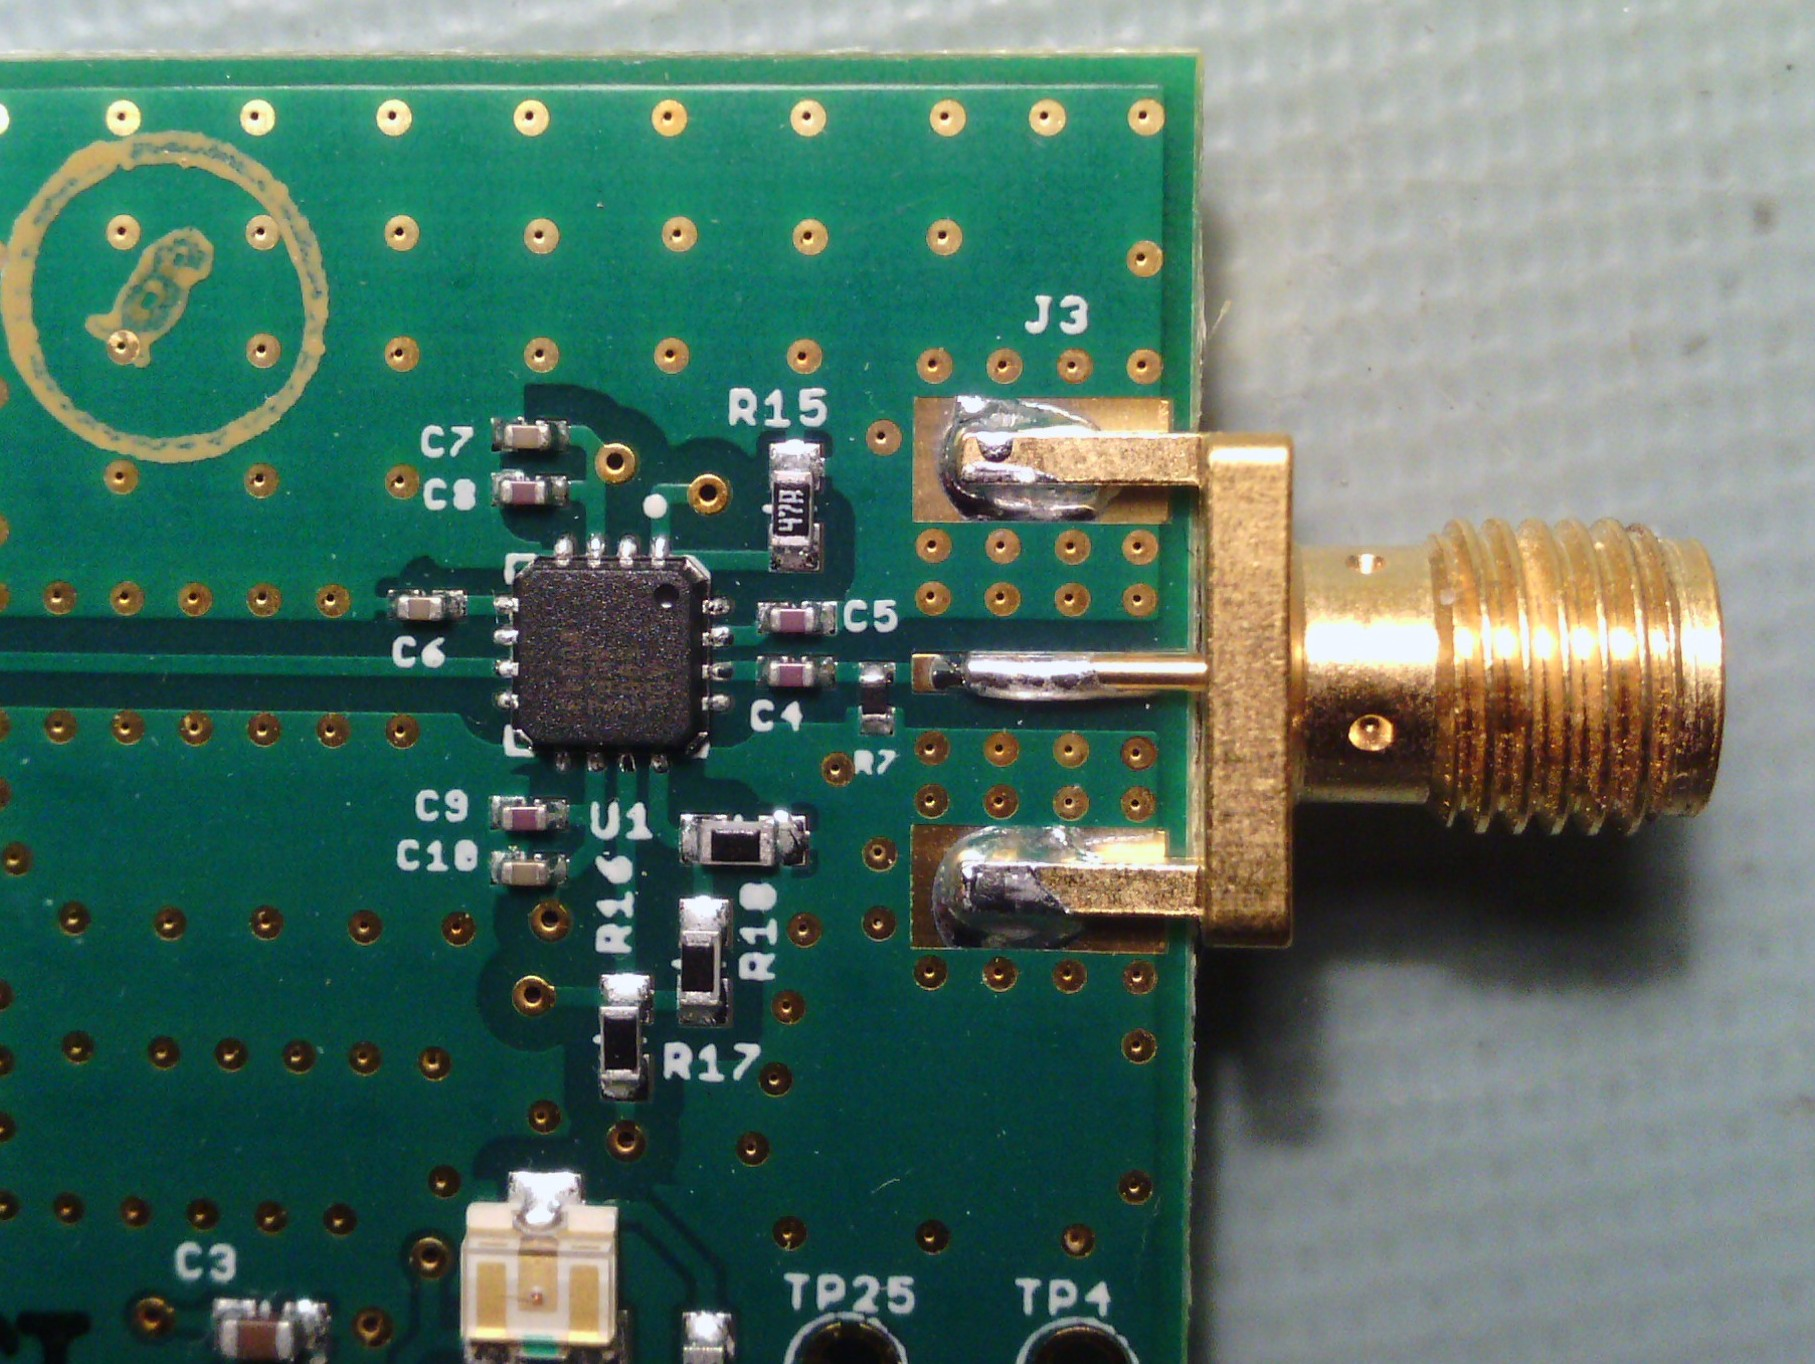
\includegraphics[width=\textwidth]{Images/adl5902.jpg}
\isucaption{An image of the ADL5902 square-law detector used in these experiments}
\label{ADL5902}
\end{figure}
}

The specifications of the ADL5902 can be seen in Table~\ref{ADL5902_data} shown below.

\begin{table}[h!tb] \centering
\isucaption{ADL5902 Specifications}
\label{ADL5902_data}
% Use: \begin{tabular{|lcc|} to put table in a box
\begin{tabular}{lcc} \hline
\textbf{Parameter @ 900 MHz} & \textbf{Value} & \textbf{Units} \\ \hline
Frequency Range & 50 to 9000 & MHz \\
Dynamic Range & 61 & dB \\
Minimum Input Level, $\pm 1.0$ dB & 60 & dB \\ 
Maximum Input Level, $\pm 1.0$ dB & 1 & db \\
Logarithmic Slope & 53.7 & mV/dB \\ 
Output Voltage Range & 0.03 to 4.8 & V \\ \hline
\end{tabular}
\end{table}

The ADL5902 outputs an analog signal that falls between 0.03 volts and 4.8 volts.  It outputs a change of 53.7 millivolt per dB detected by the ADL5902.  

\subsection{Data acquisition and storage}

In order to analyze the data, a method was developed to acquire the data and store it for later use.  For the N200 software defined radio, this is done automatically by the GNURadio program.  Both the complete signal and the power information is stored to a file for later analysis.  The square-law detector however outputs information as an analog voltage that is linearly proportional to the RF power measured.  This required a system that can capture the analog signal from the ADL5902 and then send the data to be stored.  This was accomplished by using a National Instruments USB-6009 data acquisition unit.  This unit has 8 analog inputs that can sample up to 48 ksps with a resolution of 14-bits.  This was more than adequate for our needs.  To use the USB-6009 a fairly simple Lab View program was created.  This program retrieved the information from the USB-6009 and stored the data in both Labview's binary format and in a more human friendly ASCII format.  The USB-6009 then connects to a host computer through the USB interface.  This made obtaining the data and using device fairly straightforward to use.

\subsubsection{Labview Acquisition program}

The Labview program was created to talk to the USB-6009 and then store the data.  In addition, it is able to display in real time the current readings coming from the USB-6009.  This was beneficial during testing of the program but is also good information to have while running an experiment.  

{\begin{figure}[h!tb] \centering
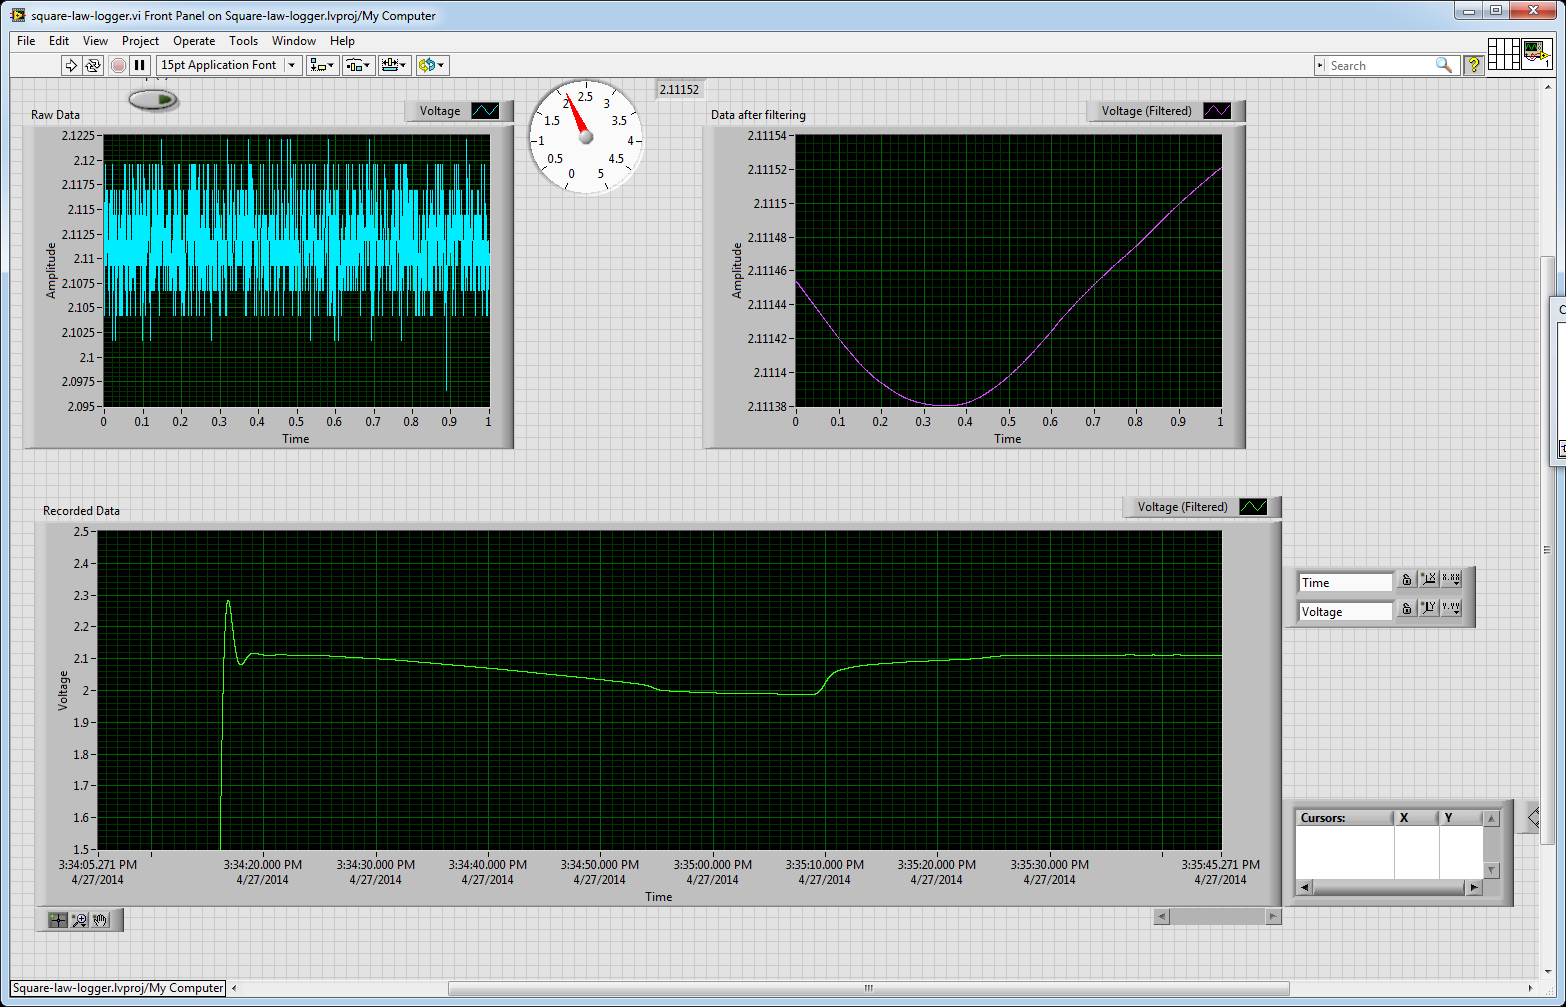
\includegraphics[width=\textwidth]{Images/labviewGUI.png}
\isucaption{A screenshot of the Labview GUI interface}
\label{labviewgui}
\end{figure}
}

The Labview program uses National Instruments DAQ assistant which allows for quick configuration and setup for the computer to talk to a number of NI devices.  Labview also includes blocks that allows us to easily record the data to a file.  These blocks made up most of the program and resulted in a program that was quickly made.  

While the USB-6009 allows up to 48,000 samples per second, we don't need such a high rate.  A rate of 1,000 samples per second was determined to provide more than enough samples of data.  With such a high rate of samples however, the resulting output will be noisy due to the natural noise found in the RF signal.  Like the software defined radio, we want to filter this noise as well to produce a smoother output.  This was accomplished using a filter block in Labview to help reduce the noise.

{\begin{figure}[h!tb] \centering
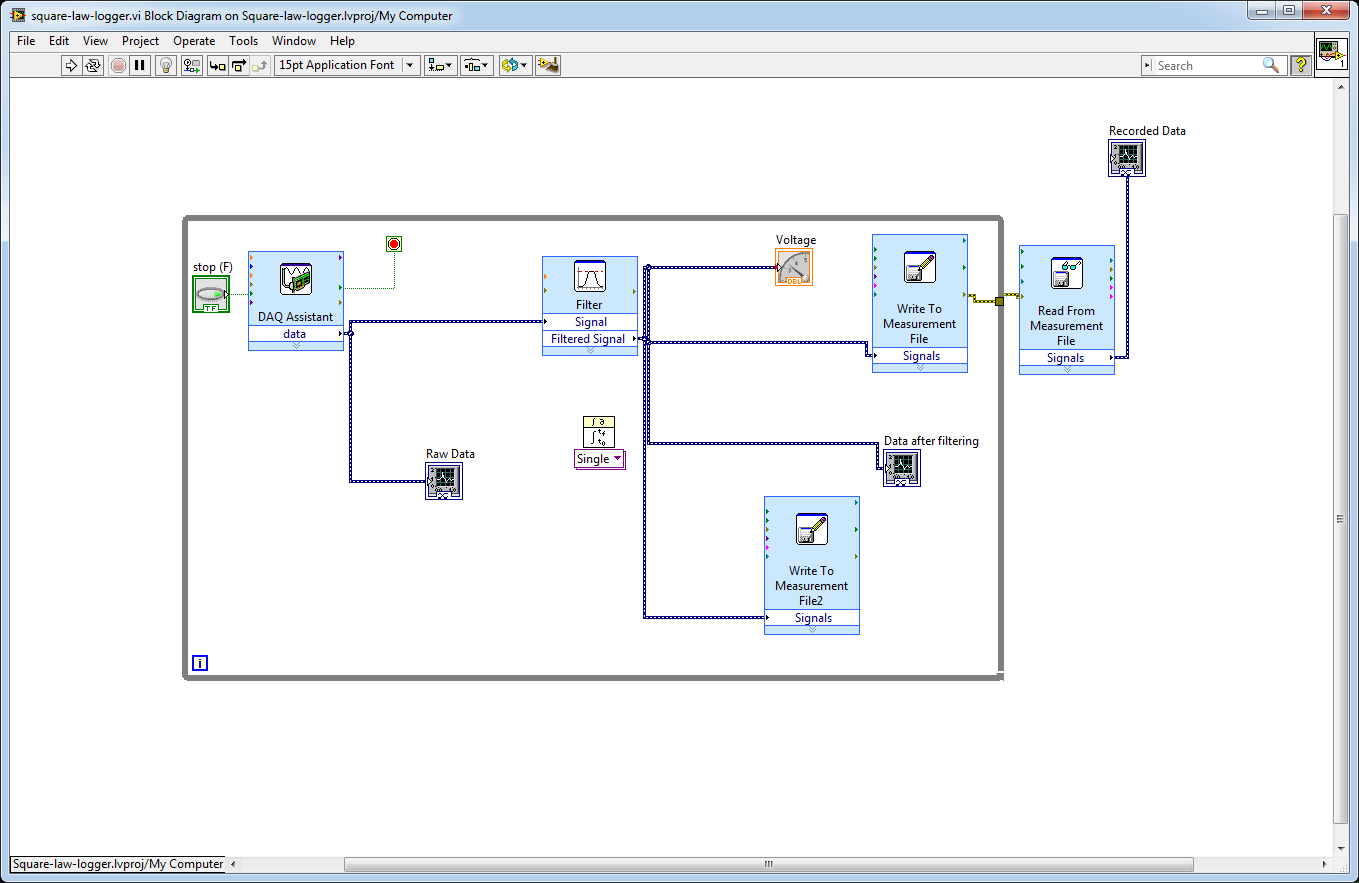
\includegraphics[width=\textwidth]{Images/labview-diagram.png}
\isucaption{A screenshot of the Labview block diagram}
\label{labviewblock}
\end{figure}
}

This program allowed for the data from the square law detector to be easily recorded.  Using Labview also allows us to customize the interface more to our liking and other features such as adding calibration information can also be added as well.  

\subsection{Tests on the ADL5902}
To test the ADL5902 a signal generator was used that had a controlled output.  The specific signal generator that was used was an older model that allowed us to change the output in 10 dBm increments.  The signal generator was also configured for 1.4 GHz as that is the frequency the ISU RF front end is configured to listen at.  Ideally a noise generator would have been desirable, however a noise generator with adjustable power output could not be located on campus.  

The ADL5902 is available from Analog Devices in an evaluation board.  This board pairs the ADL5902 with a AD7466 12-bit analog to an analog to digital converter.  This board can then be mated with Analog Devices BlackFin processor which acts as a USB gateway for the AD7466 data.  A test program written in LabView is also provided as well.

The test program provided by Analog Devices allows us to query the ADL5902 and record the raw ADC value.  The test program also allows us to enter in the frequency used during testing and the temperature during the test.  The test program also allows us to calibrate the system as well.  All of the data is then stored into an Excel spreadsheet which can be accessed later.

For this test we used the signal generator set to 1.4 GHz and started at $-60$ dBm for the output signal.  This was selected as this is the lowest the square law detector can detect.  The output power was then incremented on the signal generator in 10 dBm steps.  There was no change to any other parameter.  This was done up to 0 dBm.  Any higher and there was risk of damage to the ADL5902.  This test was then repeated several times and was done with the signal generator stepping up from $-60$ dBm to 0 dBm and from 0 dBm to $-60$ dBm.  

The data collected was then graphed using Excel.  The graph shown in~\ref{adl5902_linear}
Shows that the ADL5902 has a linear output and matches the expected value based on the input.  

\begin{figure}[h!tb] \centering

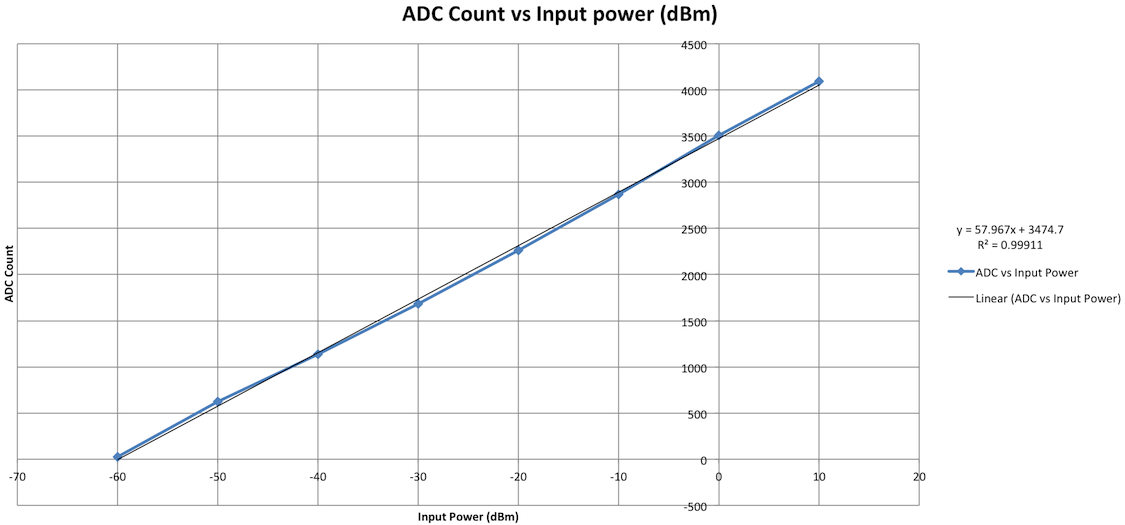
\includegraphics[width=\textwidth]{Images/Linearsquarelaw}

\isucaption{Graph showing the linearity of the ADL5902}
\label{adl5902_linear}
\end{figure}

Once it was confirmed the ADL5902 does in fact have a linear response, we then looked at ways to work with the ADL5902.  The graph above was generated using Analog Devices program that talked to the Blackfin processor on the daughter-board.  However, the information for talking to the Blackfin is proprietary.  Therefore the daughter-board was removed for future tests and instead we used the USB-6009 data acquisition board to read the raw analog voltages from the ADL5902.  This information was then stored later for additional analysis.  

\section{Software Defined Radio Experiments}
Once it was confirmed that the square-law detector was working within the specifications that were given, testing then moved to the software defined radio.  Once the Python program was established for replicating a total power radiometer in software, this was then loaded into GNURadio and used to control the N200 SDR.  

Before testing the program with the N200, testing was done with the built in noise generator in GNURadio.  This was used to test it's ability to measure small changes in noise.  This simulated noise verified that the program written was able to detect changes in noise power using a simulated Gaussian source.  It was also desired to also use a hardware based noise generator, however a suitable noise generator could not be located on campus.

{\begin{figure}[h!tb] \centering
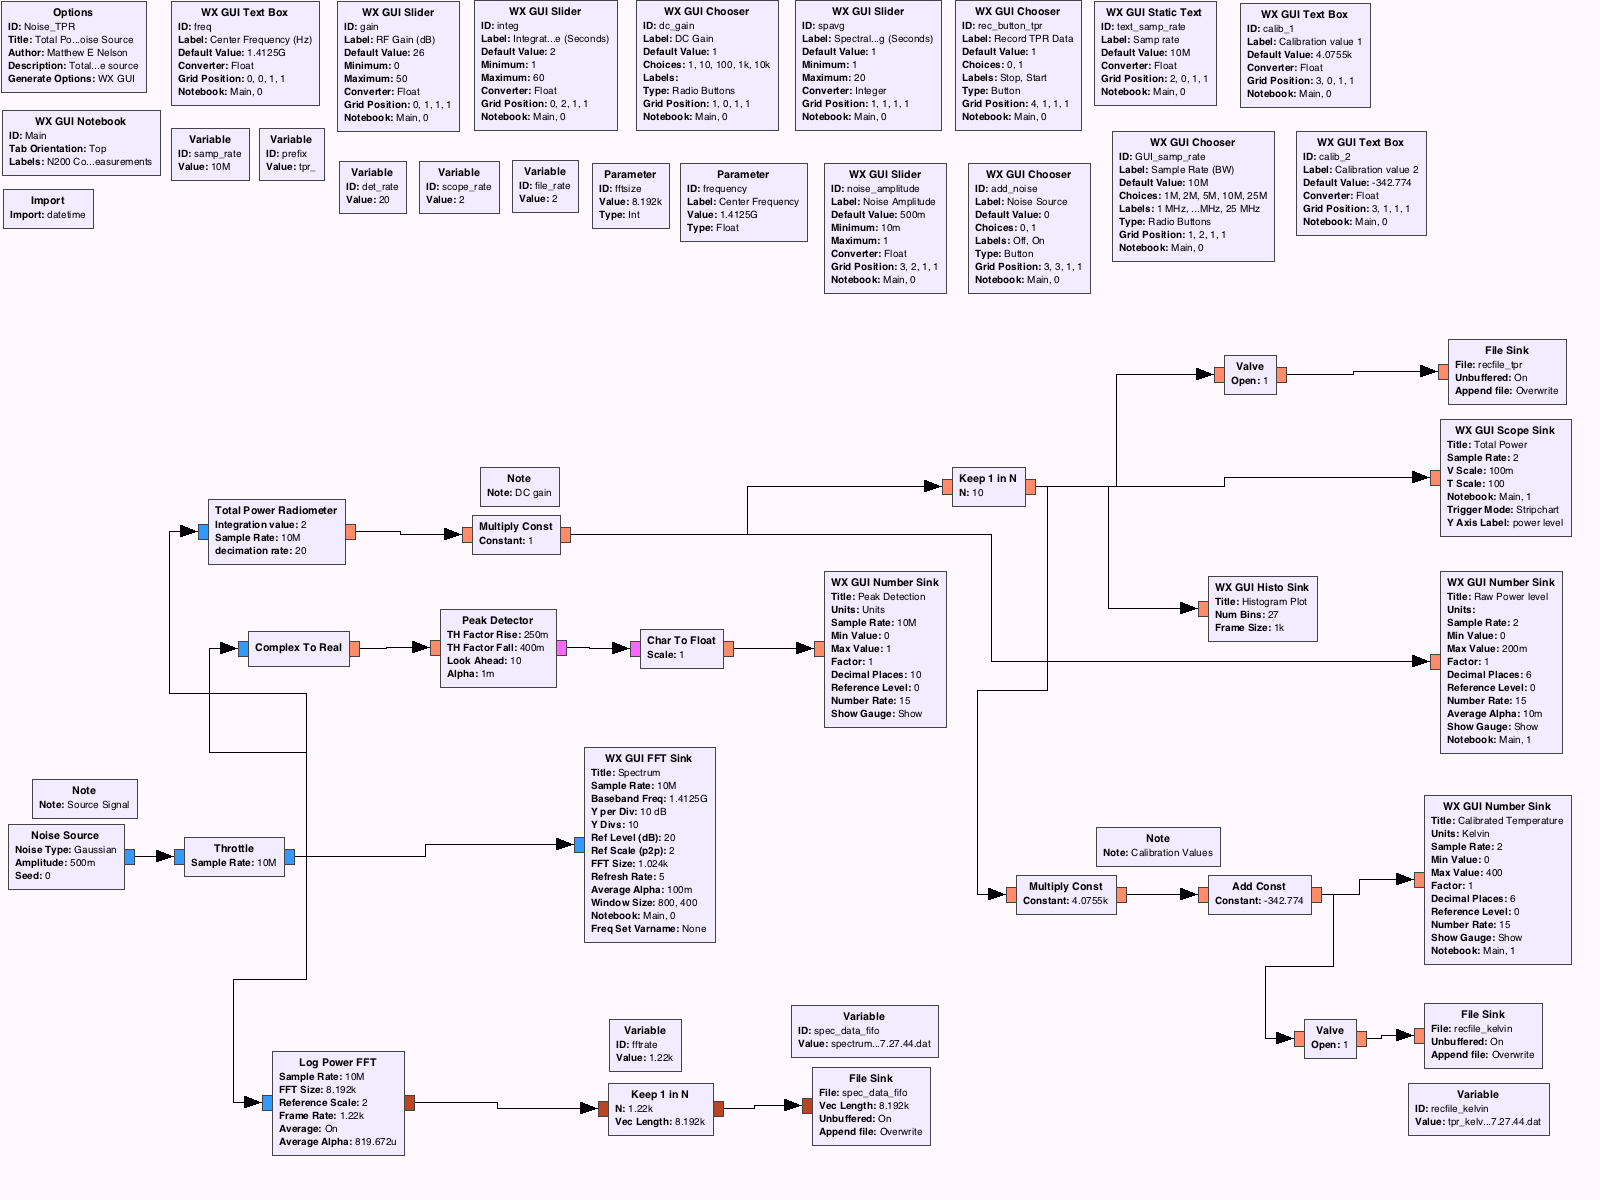
\includegraphics[width=\textwidth]{Images/noisesrc_radiometer.png}
\isucaption{A screenshot of the GNURadio program using a noise generator block.}
\label{noise_test}
\end{figure}
}

After this was done additional tweaks were made to both the GUI interface and to the program that performs the calculations for the total power radiometer.  The essential components were moved to a custom block which helped to clean up the block diagram.  Details on how this works was discussed in chapter three.

Three experiments were conducted to verify the operation of the software defined radio.  One experiment that tested stability will be discussed in chapter 5.  The other two experiments will be discussed in detail here.  These two experiments verified that the software defined radio behaved in a similar fashion to the square-law detector and also demonstrated an additional function that the square-law detector was not able to do.

\section{Experiment 1 - Calibration and Normal Radiometer Operation}

To fully test both the total power radiometer in the software defined radio and the square-law detector, a cold water bath experiment was established to verify that both the square-law detector and SDR was able to measure real world changes in the noise.  In addition, this would also give us a calibration line to to calibrate the radiometer.

\subsection{Laboratory Setup}
For this experiment the, ISU radiometer was setup in the Make to Innovate lab located in Howe Hall at Iowa State University.  This lab was picked as it has a an electronics area and has test equipment needed for certain experiments as well as the needed power supplies to power the equipment.  To measure the change in noise, a 50 ohm matched load was attached to the input of the LNAs and this output was then feed to a power divider which divides the signal between the software defined radio and the square-law detector.  This does add a 3.1 dB loss to both devices, however this was acceptable for these experiments.

\begin{figure}[h!tb] \centering

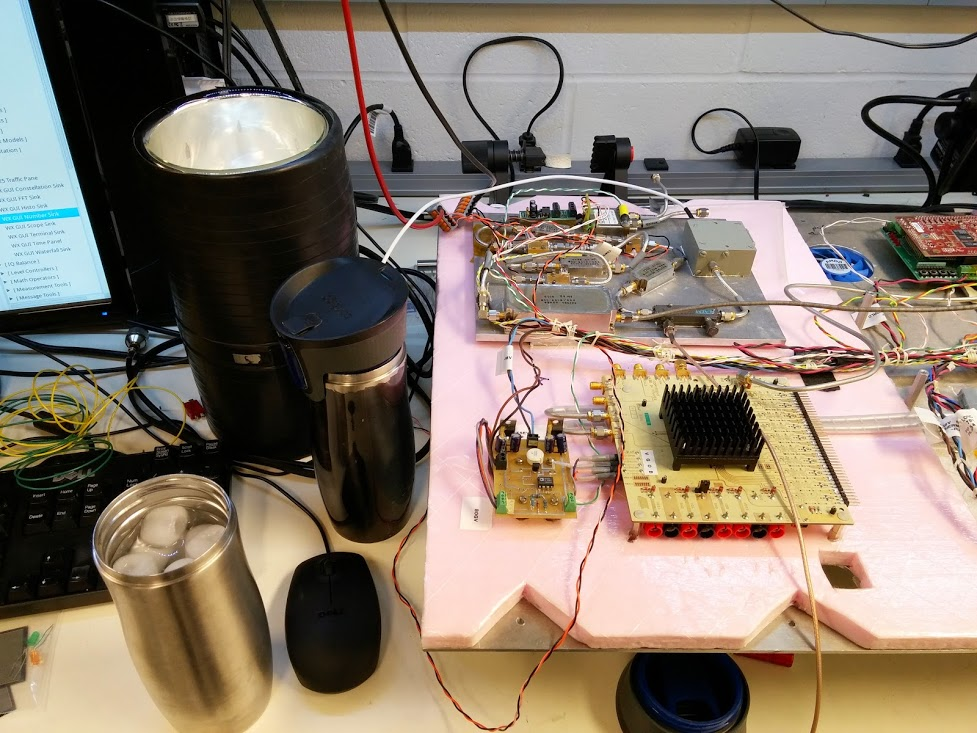
\includegraphics[width=\textwidth]{Images/exp1_setup.jpg}

\isucaption{An image of the typical lab setup used to test the software defined radiometer}
\label{LabSetup}
\end{figure}

The 50 ohm load was then submersed into a hot or cold bath.  These baths were temperature controlled first by using Liquid Nitrogen (LN2) which is known to boil at 77 K and an ice water bath which is known to be at 273.15 K.  The temperature of these could easily be monitored and maintained.  The load was submersed in each bath for a minimum of 2 minutes to allow for it to reach the same temperature as the bath.  The noise measured was then recorded using GNURadio with the N200 SDR and with the USB-6009 to record the square-law data.  In addition to the total power measurements, the raw I-Q data was also recorded.  This allowed us to replay the experiment through GNURadio for further study.
\subsection{Test Results}

The first data we will look at with be with the software defined radio.  The SDR records the total power measurements to a binary file that either Matlab or Python can read.  In our results, we used iPython Notebook to read and generate the graphs used in this thesis.  We will begin by looking at the raw total power readings which we will call raw Q values or rQ values.  These are the uncalibrated total power readings from the software defined radio.  

\begin{figure}[h!tb] \centering

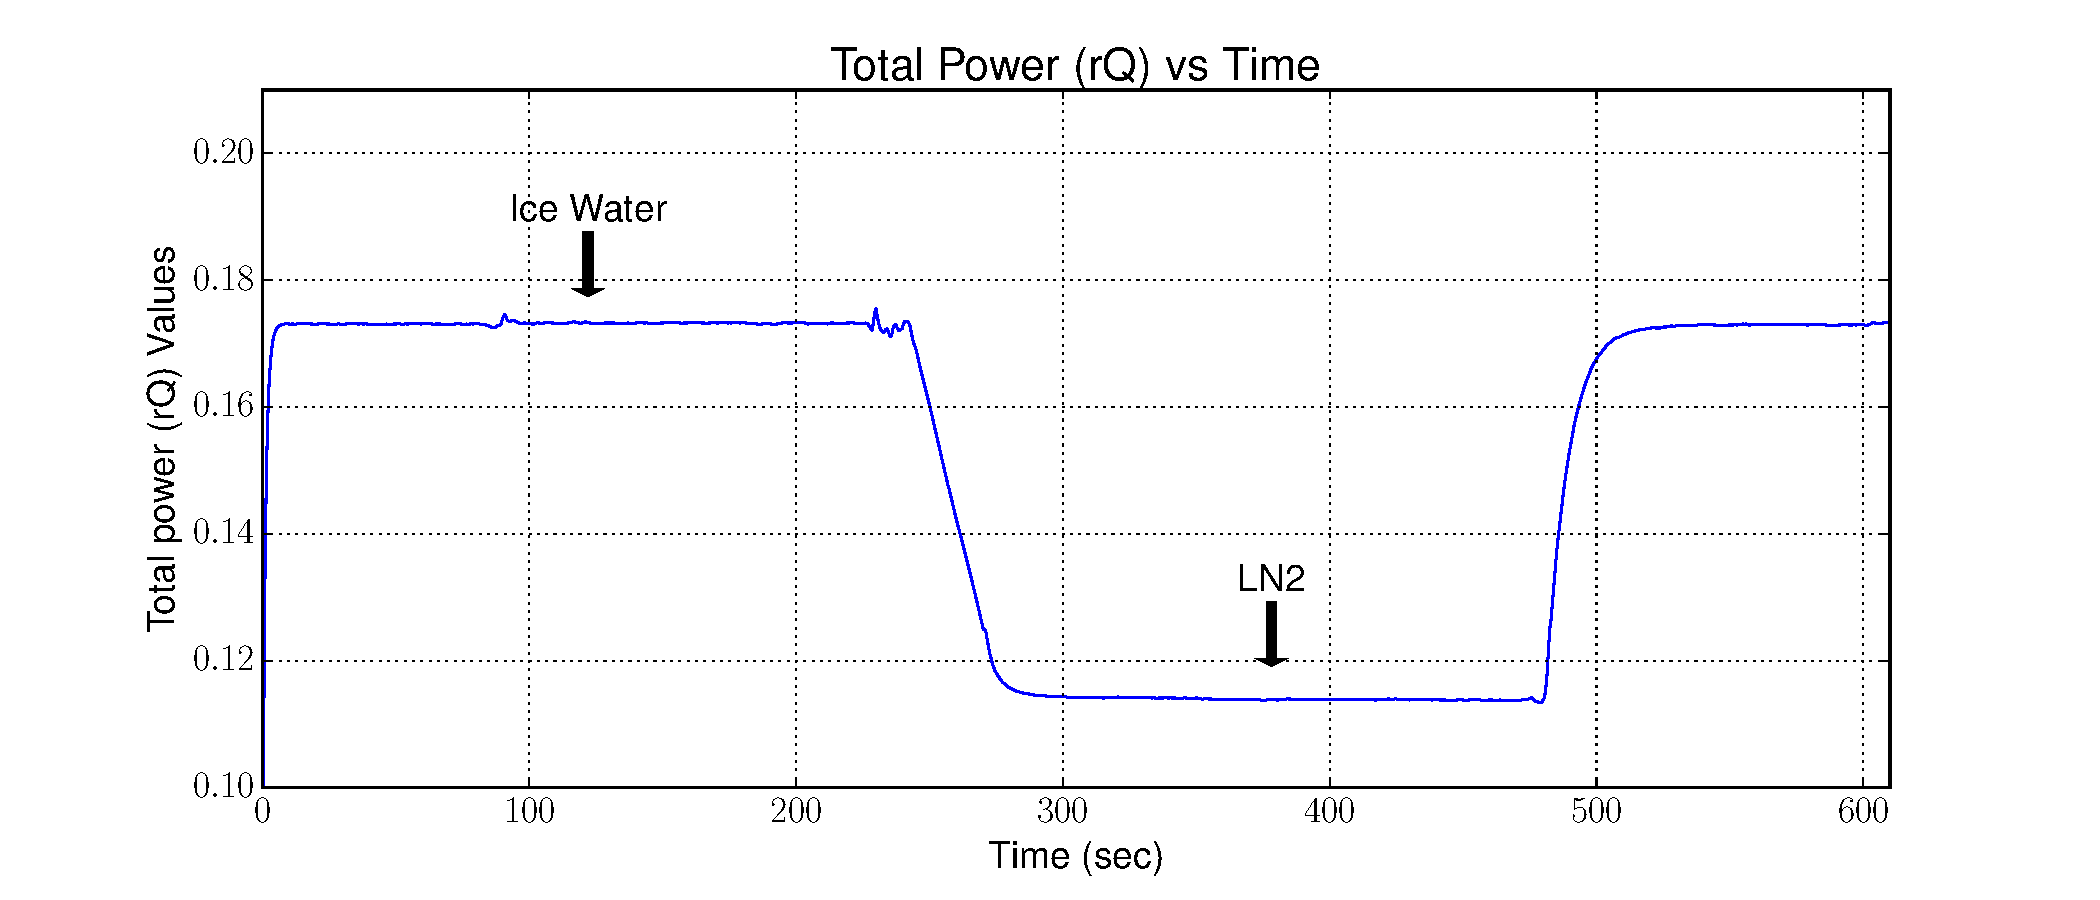
\includegraphics[width=\textwidth]{Experiments/Exp1/rqvstime_annotate.pdf}

\isucaption{Graph of the un-calibrated rQ values of Experiment 1}
\label{SDR_rQ}
\end{figure}

Figure \ref{SDR_rQ} shows the total power reading versus time and is also marked when the matched load was submerged in Ice Water, LN2, or a hot water bath.  Since we know what the temperatures are for the ice water and LN2, we can now calibrate these readings to a noise temperature reading.  This is done by reading in a calibration file we have stored in csv format and performing linear algebra to solve the slope of the line.  This was done in our iPython Notebook using the following code.
\lstset{language=Python}
\begin{lstlisting}[frame=single,keywordstyle=\color{blue}]
a = numpy.array([[rQ_values[0],1.0],[rQ_values[1],1.0]],numpy.float32)
b = numpy.array([temp_values[0],temp_values[1]])
z = numpy.linalg.solve(a,b)
\end{lstlisting}

Now that we have our calibration points, we can now re-graph this data but now have it reference the noise temperature. Figure \ref{SDR_Calibrated} shows a calibrated graph of the data in relation to noise temperature.  In addition we have colorized this graph to show "warmer" to "cooler" temps.  This is helpful as we often refer to these as noise temperatures.

\begin{figure}[h!tb] \centering

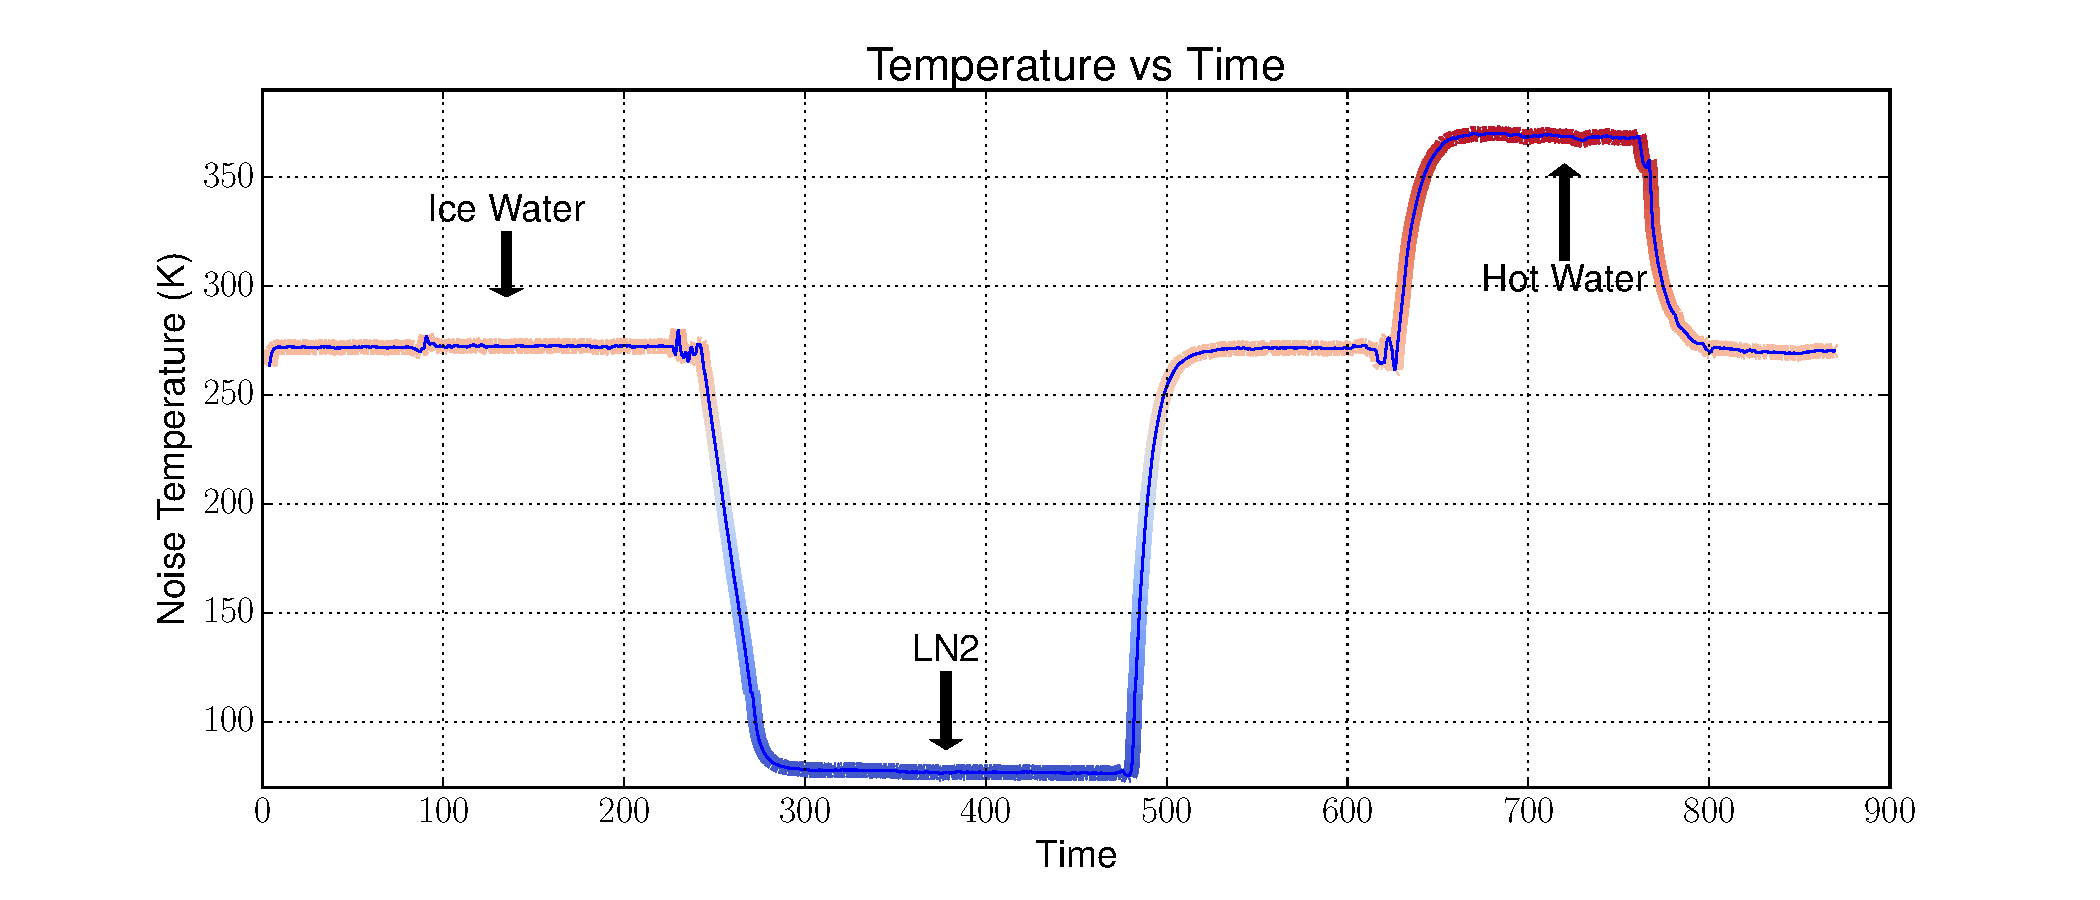
\includegraphics[width=\textwidth]{Experiments/Exp1/sdr_calibrated_color.pdf}

\isucaption{Graph of the calibrated noise temperature of Experiment 1}
\label{SDR_Calibrated}
\end{figure}

Now that we have looked at the software defined radio data, we want to look at the square-law detector with the end result of comparing the two.  The square-law detector gives us power information as a voltage, so once again we will need to calibrate this to the known temperature references.  However, before that we need to do one other step with the data.  Unlike the software defined radio, there is no filter or integrator to help smooth out the data, so the square-law data is very noisy.  Our first step will be to filter the data.  Figure \ref{X2_Raw} shows our raw data that we get from the square-law detector.

\begin{figure}[h!tb] \centering

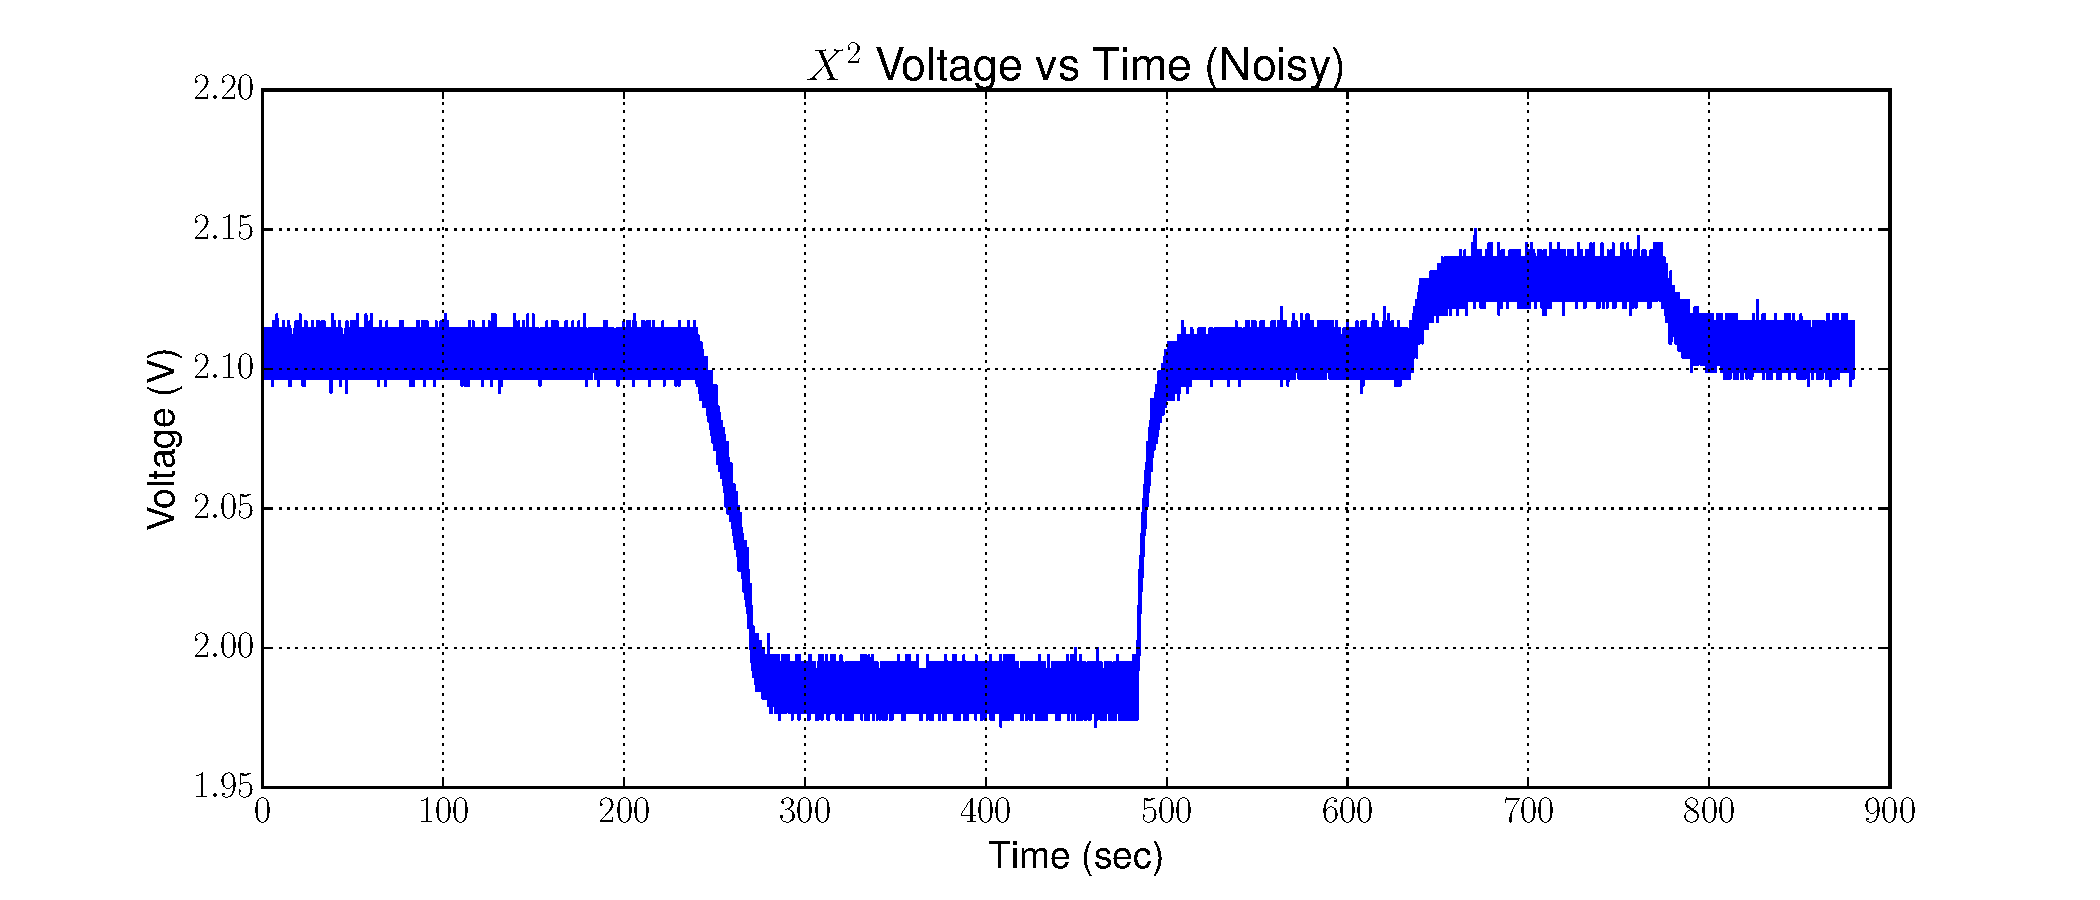
\includegraphics[width=\textwidth]{Experiments/Exp1/noisy_voltage.pdf}

\isucaption{Raw and noisy graph from the square-law detector used in Experiment 1}
\label{X2_Raw}
\end{figure}

Once again we can use Python to process this information and specifically we can use SciPy which includes several useful signal processing modules.  For our use, we will use a low pass filter to clean up the signal.  The following code allows us to do just that.

\begin{lstlisting}[frame=single,keywordstyle=\color{blue}]
from scipy import signal
N=100
Fc=2000
Fs=1600
h=scipy.signal.firwin(numtaps=N, cutoff=40, nyq=Fs/2)
x2_filt=scipy.signal.lfilter(h,1.0,x2_voltage)
\end{lstlisting}

Figure \ref{X2_filter} now shows our data that has been filtered by the low pass filter.  This is similar to the low pass filter that is also used by the software defined radio.

\begin{figure}[h!tb] \centering

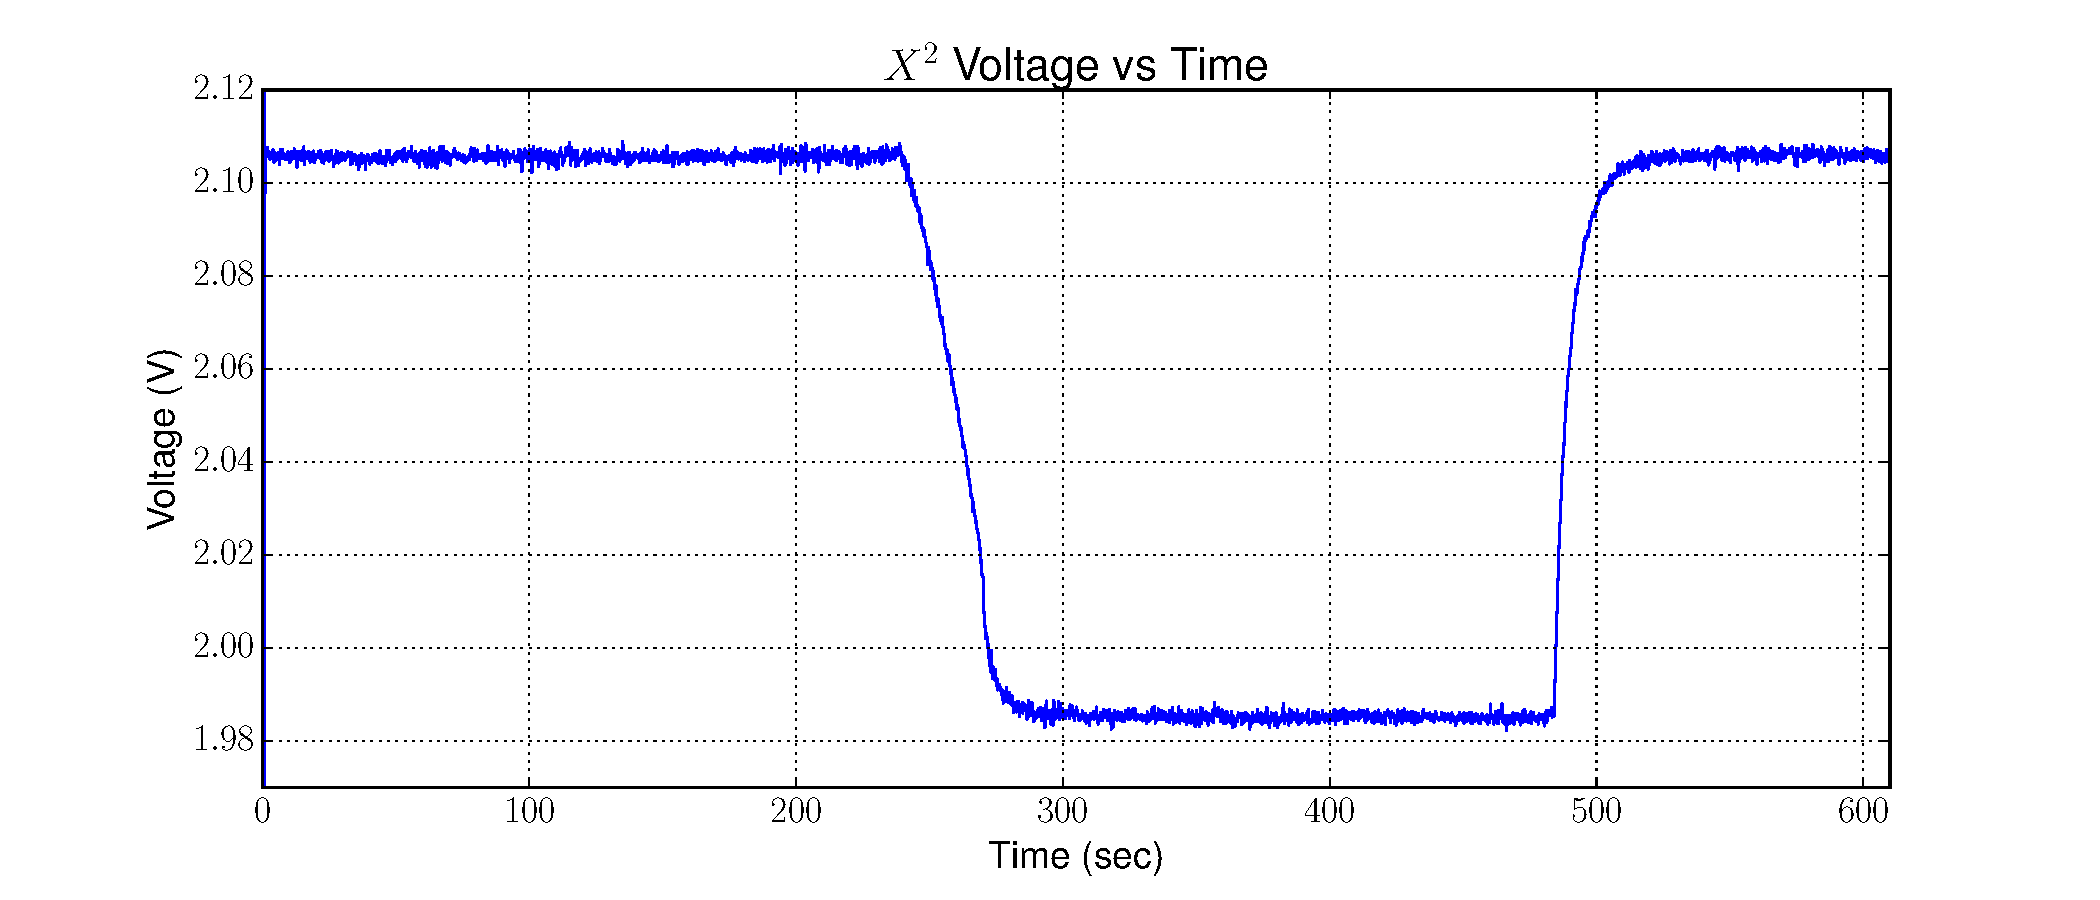
\includegraphics[width=\textwidth]{Experiments/Exp1/x2_filter.pdf}

\isucaption{Filtered data from the square-law detector used in Experiment 1}
\label{X2_filter}
\end{figure}

Using the same technique as earlier, we can now calibrate the raw voltages from the square-law detector to the noise temperature.  Like the software defined radio data, we can calibrate the voltages from the square-law detector to the physical temperature that our matched load is placed in.  Figure \ref{X2_Calibrated} shows the data from the square-law detector calibrated to our known temperature points.  This now allows us to to directly compare the square-law detector to the software defined radio data since we have a common reference point in which to compare the data.

\begin{figure}[h!tb] \centering

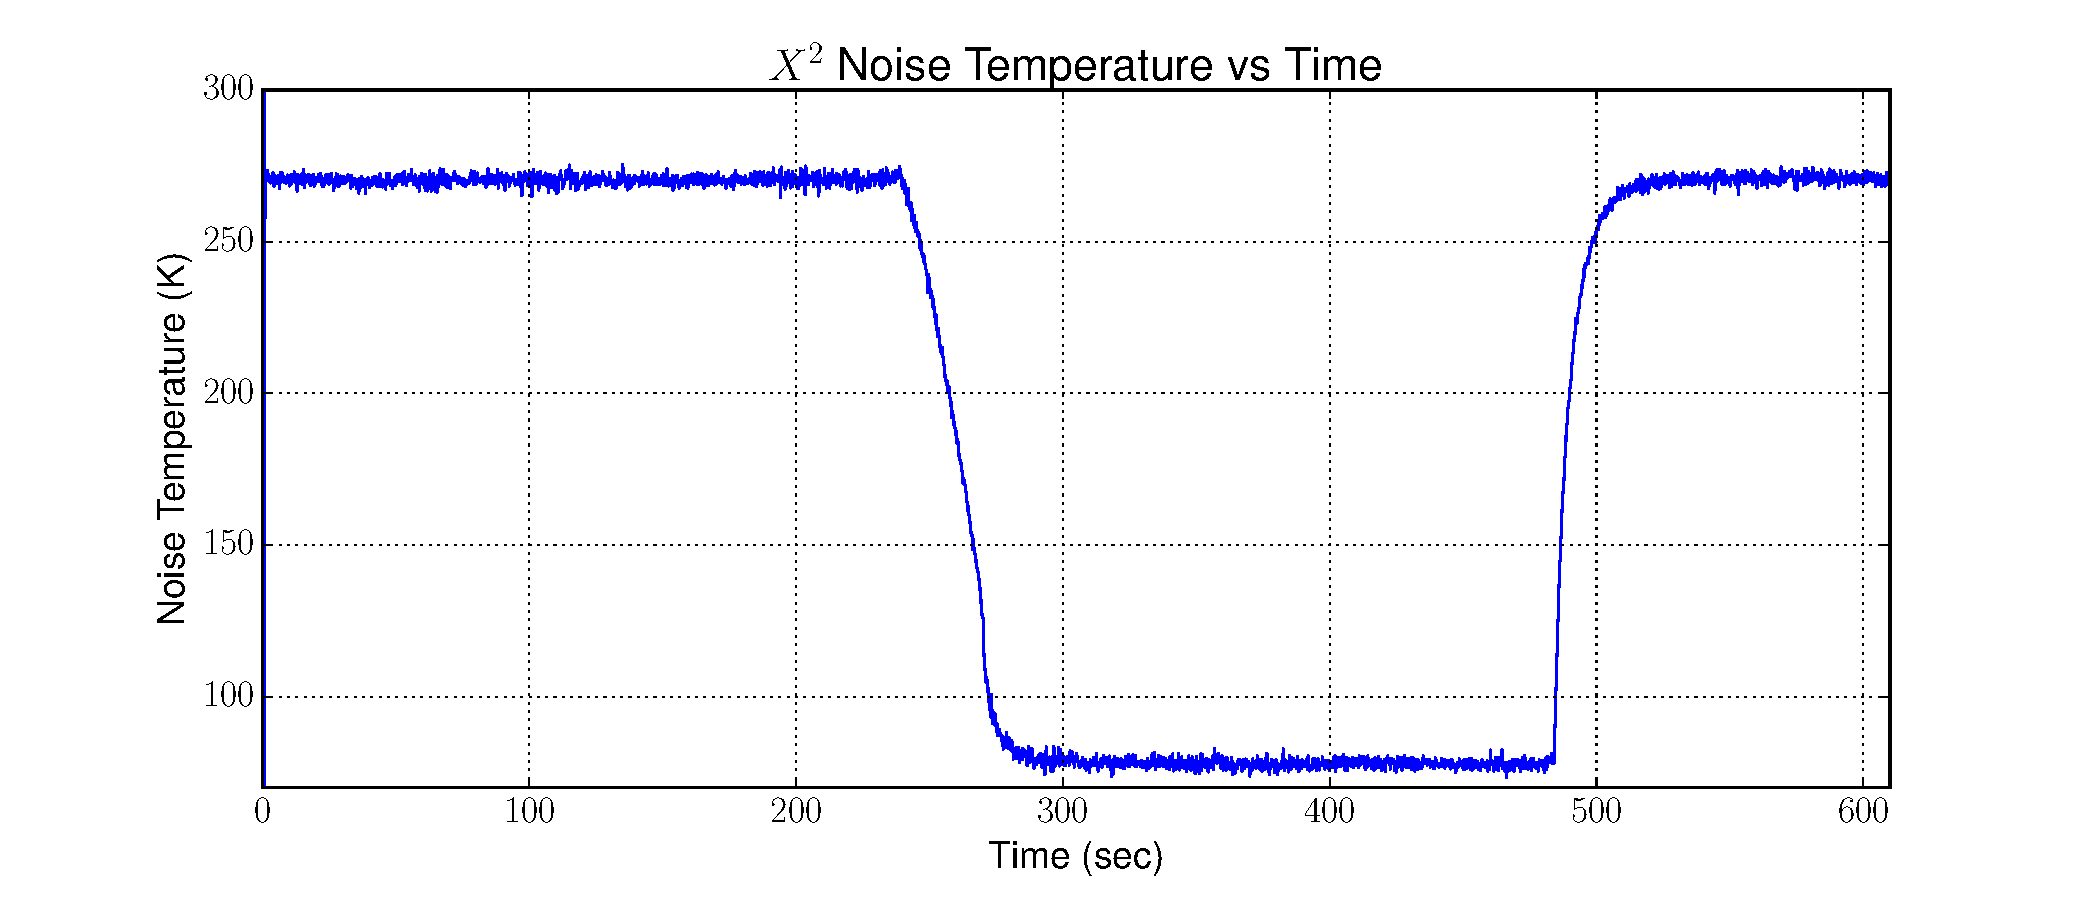
\includegraphics[width=\textwidth]{Experiments/Exp1/x2_calibrated.pdf}

\isucaption{Calibrated data from the square-law detector used in Experiment 1}
\label{X2_Calibrated}
\end{figure}

We now want to compare both the Software Defined Radio and the square-law to make sure that they match up.  Since both the SDR and the square-law are now calibrated to a noise temperature, we can easily graph both of the data and compare to see how well they match up.

\begin{figure}[h!tb] \centering

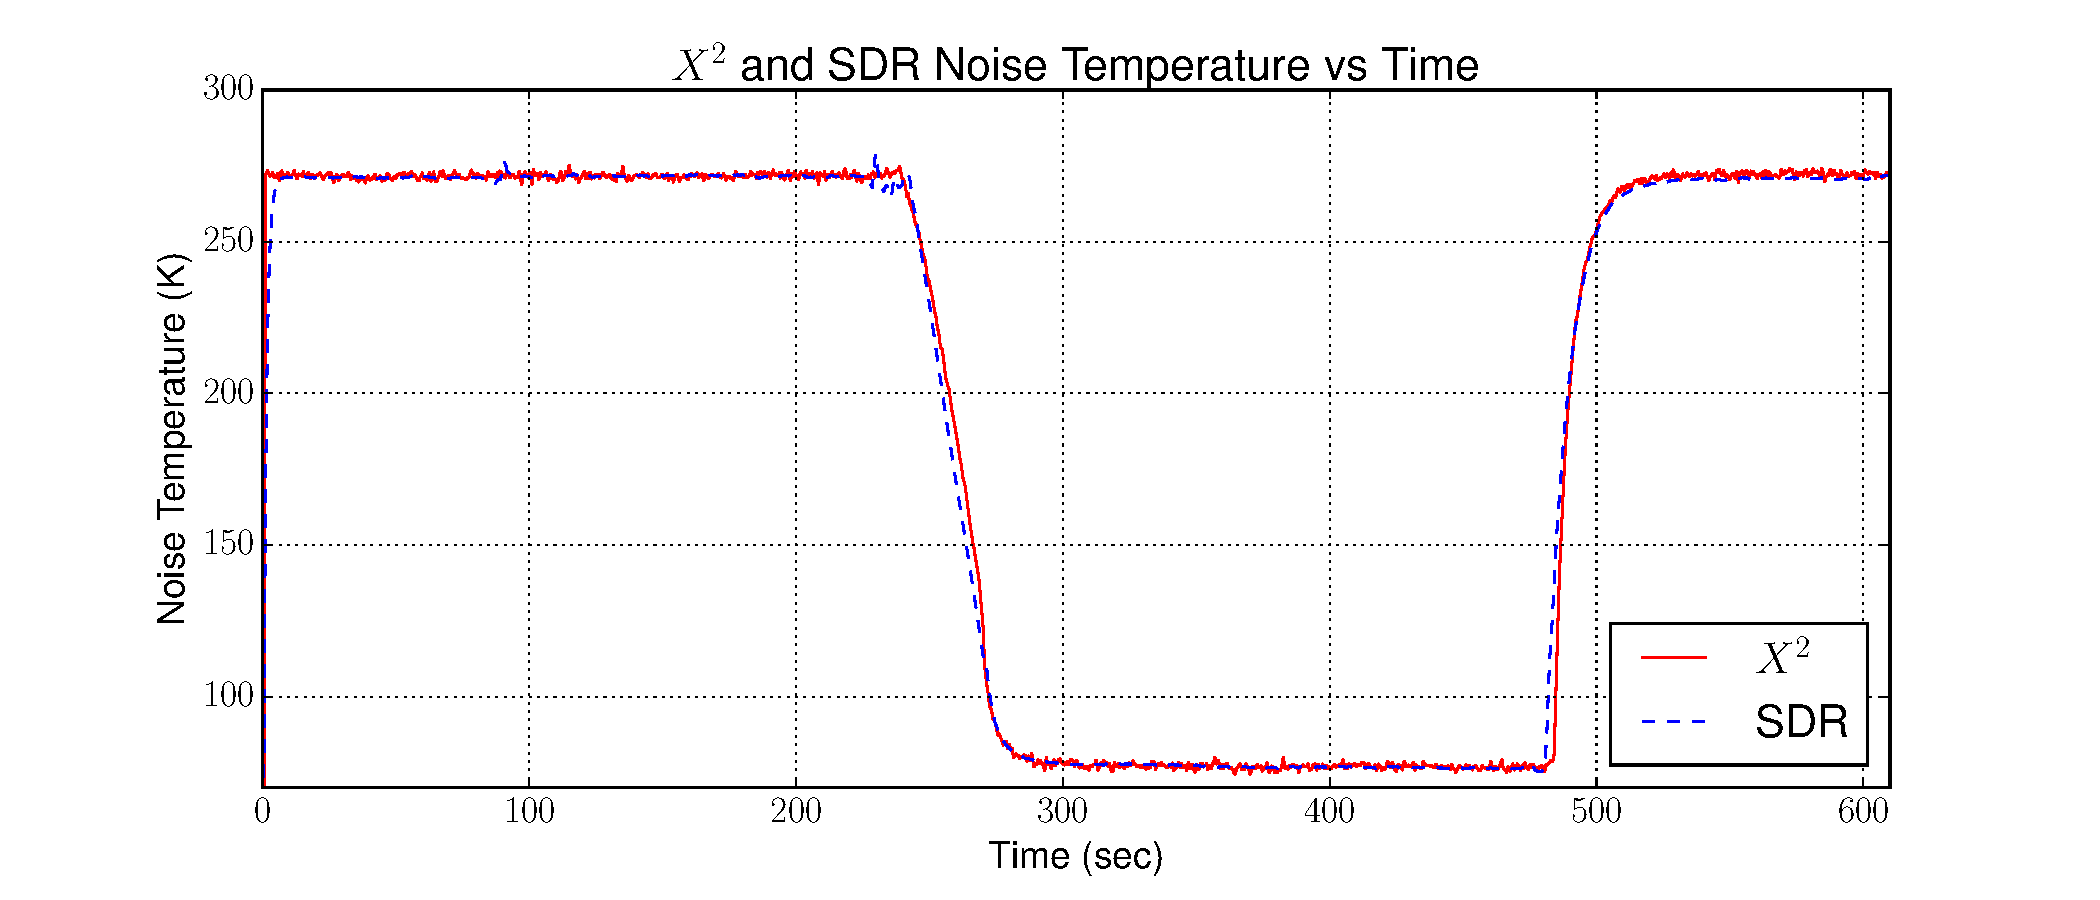
\includegraphics[width=\textwidth]{Experiments/Exp1/x2_SDR_Calibrated.pdf}

\isucaption{Figure showing both the SDR and square-law noise temperature data in Experiment 1}
\label{X2_SDR_Both}
\end{figure}

We can see in Figure \ref{X2_SDR_Both} that both the software defined radio and the square-law detector match up very nicely.  This shows that both the square-law detector and the software defined radio agree when properly calibrated.  This verifies that the software defined radio can indeed operate as a total power radiometer and the data we obtain from this setup agrees with an analog and more traditional radiometer.
\subsection{Application with Soil Moisture Readings}
A common application of radiometers is in the measurement of soil moisture.  All items naturally emit RF energy due to the random excitation by the electrons in the object.  The amount of noise that gets generated varies by temperature, but the amount that reaches the antenna varies by the amount of moisture in the soil.  If we can calibrate the radiometer to two known soil conditions, then we can measure the various levels of soil moisture in the soil.  At this time, we will simply look at the percentage of moisture in the soil, which will vary from zero percent or dry soil to one hundred percent or very wet soil.  The drier the soil, the more thermal noise we receive and the "warmer" the noise temperature.  Wet soil on the other hand attenuates the thermal noise and shows up as a "cooler" noise temperature.  

Using the Software Defined Radio, we can setup two methods to visually look at the noise temperature and thus the soil moisture percentage.  Since we do not have an antenna hooked up, we will simulate this by using two reference temperatures.  In this case the ice water bath and the LN2 that we just used and was shown earlier.  

A unique visual aid we can use with GNURadio is a waterfall display.  This display gives us information that includes frequency, amplitude and time.  It is referred to as a waterfall display due to the fact the display continually moves from top to bottom and looks like a waterfall.  Amplitude information is given by mapping the range of amplitudes to a color bar.  Frequency is given on the x-axis and time is on the y-axis.  Figure \ref{LN2_waterfall} shows a screen shot of the waterfall display in the GUI created in GNURadio Companion for this experiment.  This is the same program we have used but with the waterfall display now added.  The data for the waterfall is pulled directly from our source block or in our case the N200 software defined radio.

\begin{figure}[h!tb] \centering

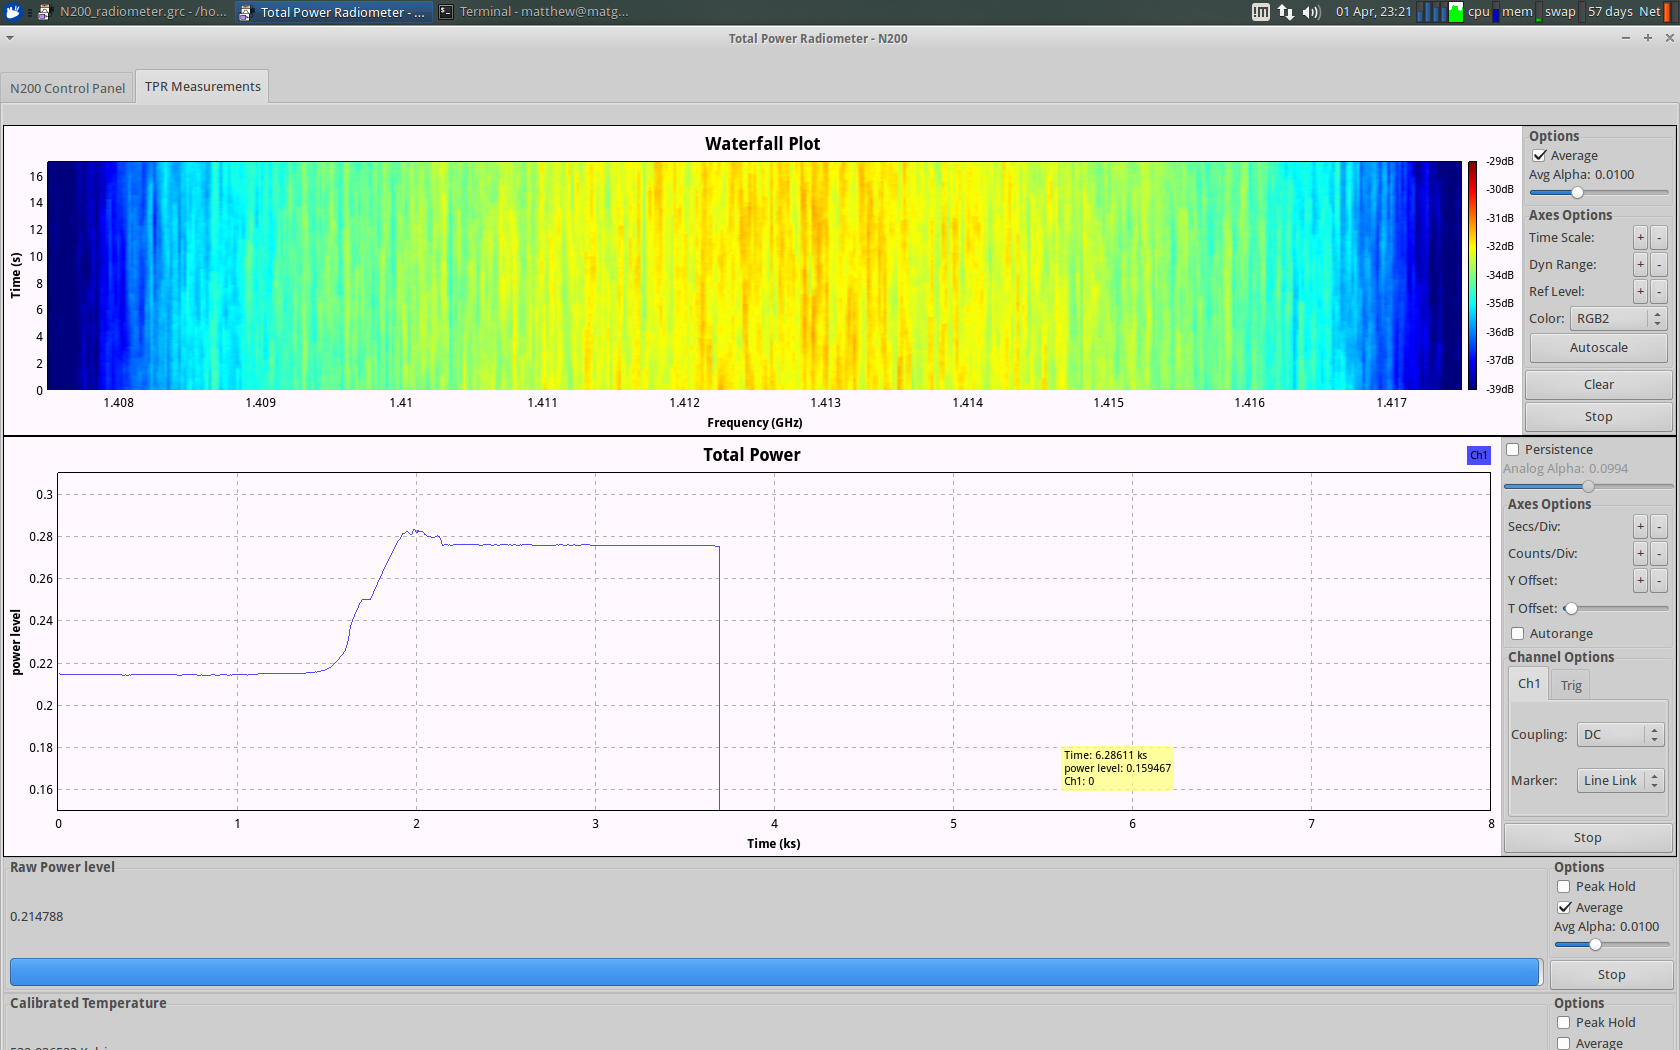
\includegraphics[width=\textwidth]{Experiments/Exp1/LN2_waterfall.png}

\isucaption{Screenshot of the waterfall display used in Experiment 1}
\label{LN2_waterfall}
\end{figure}

Let's take a look at two screen shots of the waterfall.  We will put them side by side so we can better compare the display when the thermal load is in the ice water bath and when the load is in LN2.

\begin{figure}[h!tb] \centering

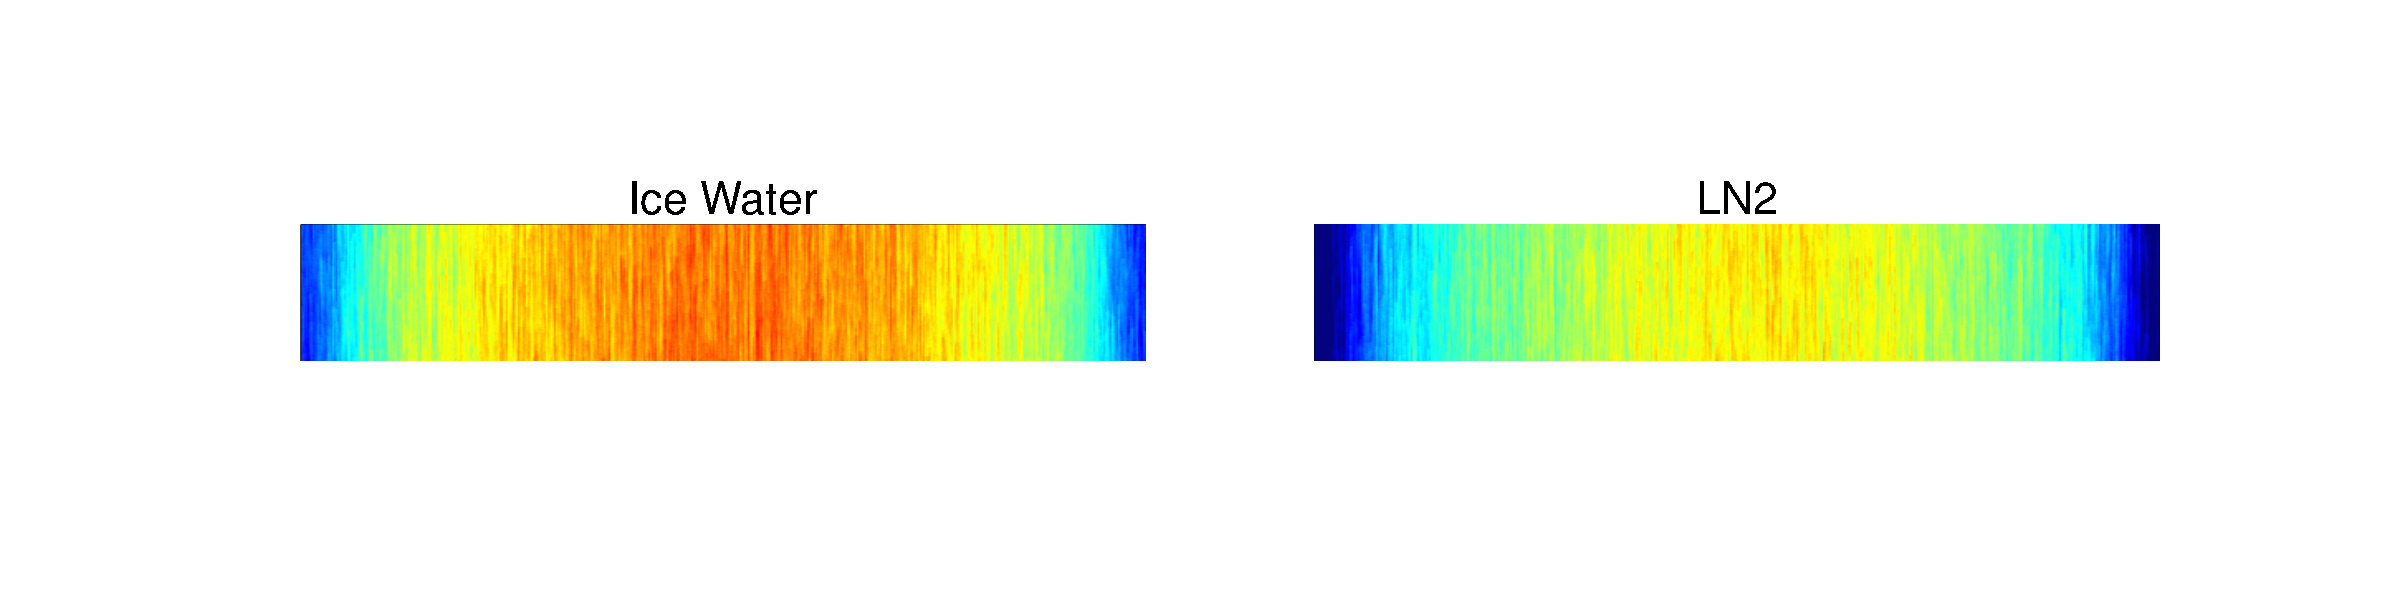
\includegraphics[width=\textwidth]{Experiments/Exp1/waterfall_side.pdf}

\isucaption{Side by side comparison of the waterfall display for Experiment 1}
\label{side_waterfall}
\end{figure}

In figure \ref{side_waterfall} we can see that the ice water screen shot appears "warmer" than the right side screen shot which appears "cooler".  There is a limitation in GNURadio and the waterfall display that limits what the range for the power readings are.  The overall power that we see only changes by about 3 dB and our current range in the waterfall display is set to 10 dB.  If we could reduce the range, the color change would be even greater and more pronounced.  However, this does show that a change can be seen visually with color to indicate the noise temperature.  

If we assume that our LN2 is dry soil and that our ice water bath is wet soil, we can now interpolate the data to this scale and show the information we obtained in Experiment one as both a noise temperature and soil moisture.  Figure \ref{SDR_soil} shows the same data we looked at earlier but we have now added a scale to show soil moisture as a percentage.

\begin{figure}[h!tb] \centering

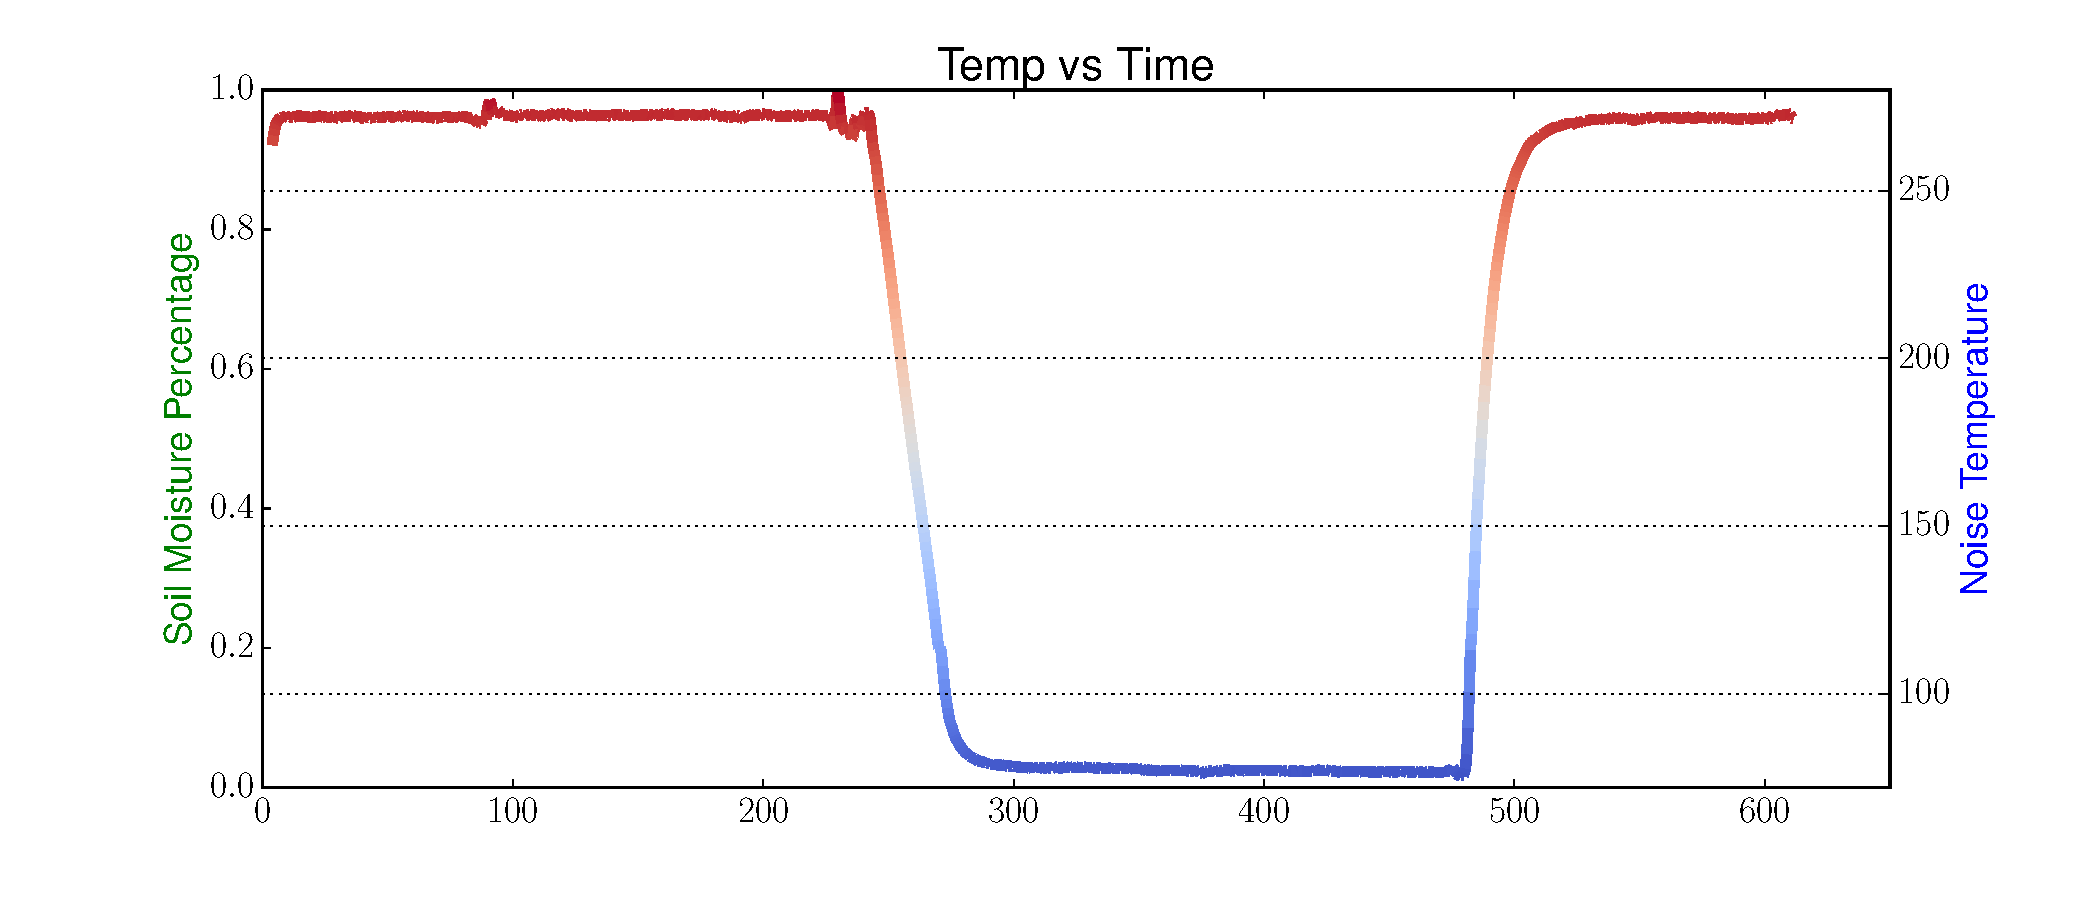
\includegraphics[width=\textwidth]{Experiments/Exp1/sdr_soilmoisture.pdf}
\isucaption{Plot of the noise temperature of Experiment 1 with soil moisture percentage}
\label{SDR_soil}
\end{figure}

While this demonstrates that we can collate our total power readings with a soil moisture percentage, we would use actual field tests to calibrate the radiometer.  In addition, we could also calibrate to soil moisture content instead of a percentage if desired.  Both methods have been done with traditional radiometers[\cite{Jonard}][\cite{Shi}.

\section{Experiment 2 - Interfering Signal Mitigation}
The addition of an unwanted signal can be a determinant to the radiometer and has an adverse affect on how the radiometer operates.  In today's world though, it is getting more difficult to control intentional radiators as the RF spectrum becomes crowded with more devices.  This problem becomes even a greater problem with radiometers used in orbiting spacecrafts as they are able to "see" large areas[\cite{DeRooRFI}].  Even though the band we are working in of 1.4 GHz is an internationally protected frequency, there can still be both intentional and unintentional radiators that cause interference.

RFI detection and mitigation is not a new topic in radiometry and there have been other methods in both the detection and mitigation of these signals[\cite{Forte}][\cite{McIntyre_RFI}][\cite{DeRoo}][\cite{Ellingson}].

Experiment 2 is used to show additional benefits of using a software defined radio compared to a more traditional radiometer by being able to filter out these unwanted signals.  One benefit of using a SDR is that key components such as filters are created in software instead of using hardware.  This means that filters can be created on the fly and can be adjusted simply by updating the software.  

For this experiment we will use both the Software Defined Radio running GNURadio with the radiometer firmware and a square-law detector that is connected to a data acquisition unit.  The experiment uses a 50 ohm matched load that is attached to the radiometer.  This matched load is then submerged into two different baths, a Liquid Nitrogen at ~ 77 K and an Ice bath at ~ 273.15 K.  Finally, for the offending signal the HackRF One is used to generate the offending signal.  This signal is generated within the 1400 to 1425 MHz that the radiometer is configured for.   for an extended period of time.  This was to determine the stability of the radiometer as it is expected that as long as the LN2 is covering the matched load, it should maintain the temperature at 77 K.  

\subsection{Laboratory Setup}
We will use a similar setup to experiment one with the addition of a signal source that we will inject into the RF chain.  Our signal source will be another software defined radio, the HackRF One shown in figure \ref{HackRF}.  This SDR is a cheaper SDR and thus has lower specifications than the Ettus Research N200.  However, for the task of a signal source, it will suit our needs.  With the exception of this additional SDR as our signal source, the setup is exactly as experiment one using the same LNAs and other hardware.

The ISU RF front end was once again used to amplify the signal.  One difference however is that a power combiner, which is the same as a power divider, was used to hook up to a signal generator.  The signal generator then provided the offending signal.  By using the signal generator we can control how much power and what frequency the offending signal is at.  In this case we are performing this in a controlled setup and would know ahead of time where the offending signal is.  In the future the SDR defined could identify the offending signal and then filter it out.

Like the other tests, a power divider is used to split the signal after the ISU RF front end which was then feed to a square-law detector and then the N200 SDR.  The square-law detector was then hooked up to a National Instruments USB-6009 DAQ.  The DAQ was then feed into a Labview program to be processed and recorded.  The N200 continued to use the GNURadio program that was created to record the total power coming out.  However, it has been modified with a band reject filter to filter the offending signal.

\begin{figure}[h!tb] \centering

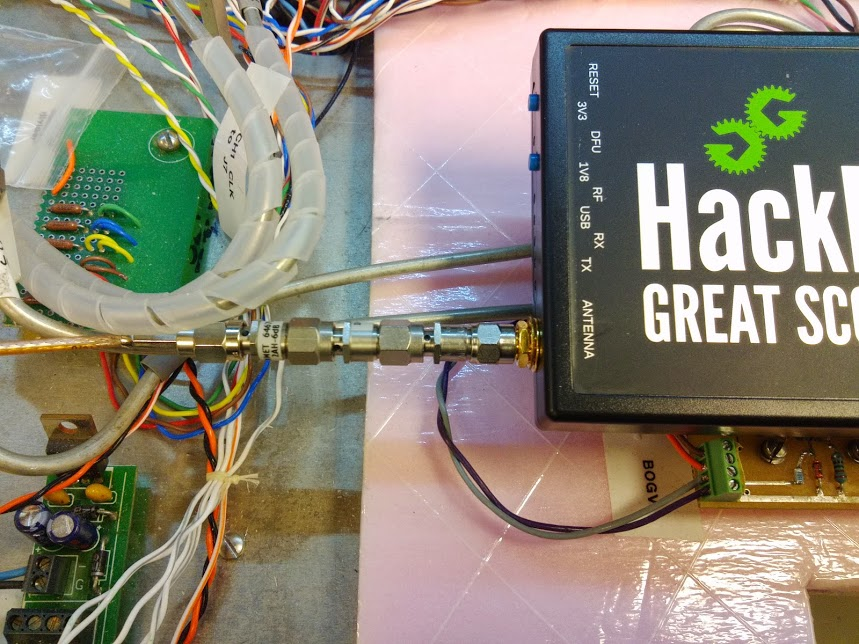
\includegraphics[width=\textwidth]{Images/Hack_RF.jpg}
\isucaption{Image of the HackRF used to generate the offending signal}
\label{HackRF}
\end{figure} 

For this experiment, the HackRF will generate a sinusoidal wave at a fixed frequency.  We will then change the amplitude of this signal a few times during the experiment.  This allows us to verify that the signal is still present in the total power measurements in both the software defined radio and the square-law detector.  Since the square-law detector does retain any frequency information, this was the only method to verify the operation of the signal generator with the square-law detector.   

\subsection{Software Defined Radio Configuration}

This test was designed to test a problem that a software defined radio would be to cope with while a square law detector would not be able to cope with it.  This test injected a known signal at 1.406 GHz to interfere with the normal operation of the radiometer.  In this test, the square law detector, since it is a wide band device, would not be able to accurately measure the change in the total power of the signal.  However, the SDR is able to create a digital filter to filter out the offending signal.  Since this is done in software, the SDR is able to adapt to changes much faster than an analog radiometer.

Our Software Defined Radio software is now altered to include a band-reject filter that will filter out the offending signal.  The filter was first designed using the included GNU Radio Filter Design tool that is part of the suite of software with GNURadio.  Figure \ref{GRC_Filter_DSN} shows a screen shot of the tool when designing the band-reject filter for this application.  This tool generates filter values also called taps that GNURadio will use for defining the filter.  The GUI program shown in figure \ref{GRC_Filter_DSN} allows us to interactively create a filter.  However, in our GNURadio program, we can call this program directly from our program to generate the taps needed.  This is quite easy to do since both GNURadio and the program that generates the taps are both Python programs.  

\begin{figure}[h!tb] \centering

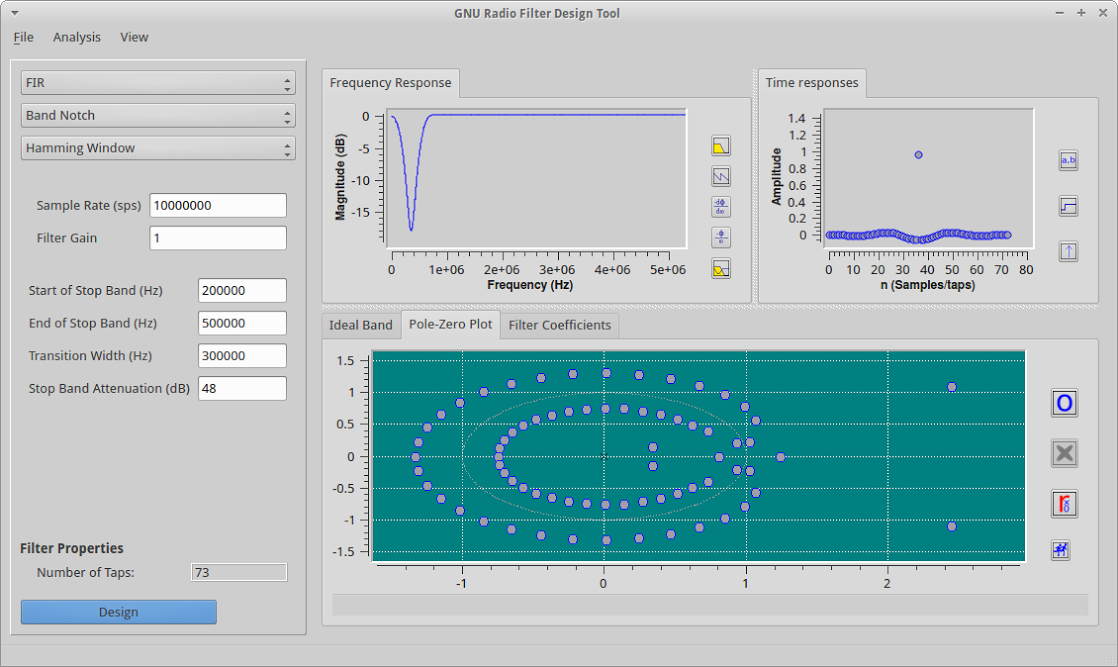
\includegraphics[width=\textwidth]{Images/GNURadio_Filter_dsn.png}
\isucaption{Image of the GNU Radio Filter Design tool}
\label{GRC_Filter_DSN}
\end{figure}  

Once we have the taps we can now apply the filter to our system.  The band-reject filter will of course affect our performance as we will lose some bandwidth to the filter.  However, as we will shortly show we are still able to function as a total power radiometer while filtering this signal.  

\subsection{Test Results}
We begin by looking at the what happens to our total power readings with no filter applied.  As we stated in the Lab Setup portion, the frequency of the offending signal will not change, but the amplitude will.  This will mean that we should see clear indications of the total power changing as the amplitude of the offending signal changes.  

\begin{figure}[h!tb] \centering

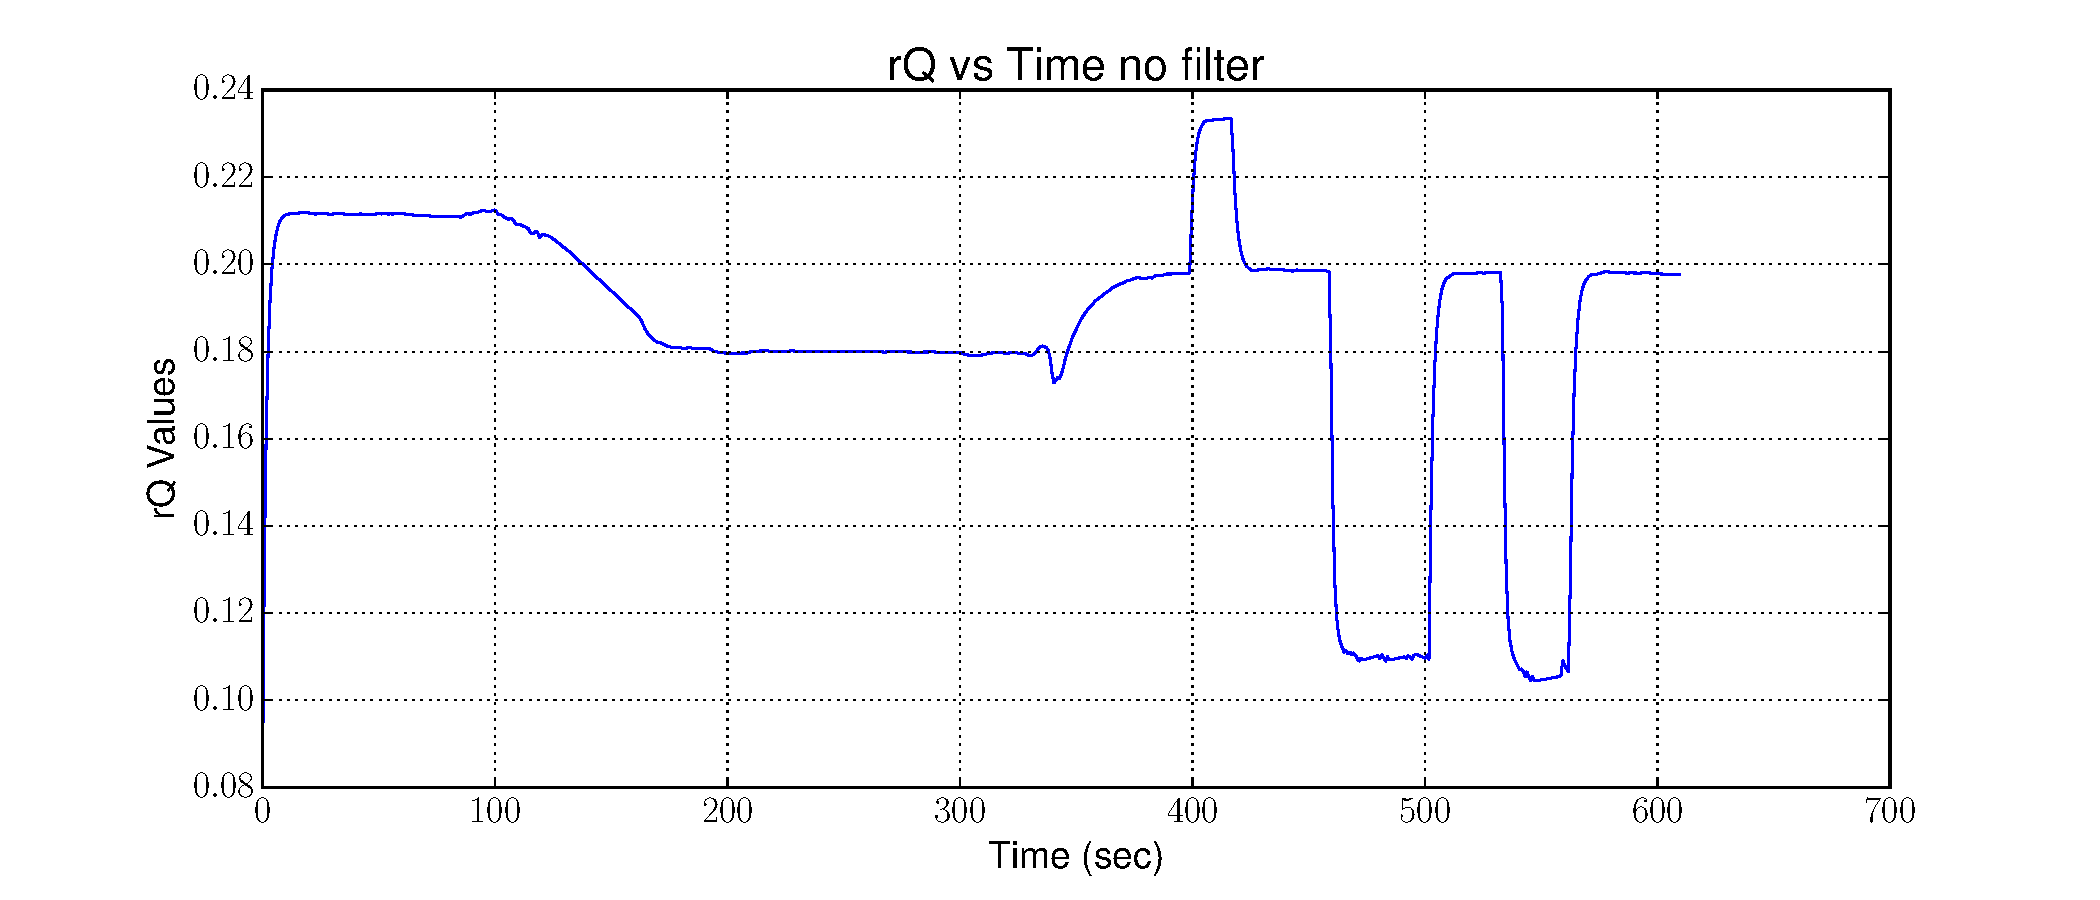
\includegraphics[width=\textwidth]{Experiments/Exp4/sdr_raw_unfiltered.pdf}

\isucaption{Graph showing the unfiltered total power measurements on the software defined radio}
\label{sdr_unfilt_raw}
\end{figure}

We can see that there are pulses that occur in the graph in figure \ref{sdr_unfilt_raw} and that changes in the amplitude of the offending signal affect our total power readings.  These same pulses can also be seen in the square-law detector data as well which can be seen in figure \ref{x2_unfilt}.

\begin{figure}[h!tb] \centering

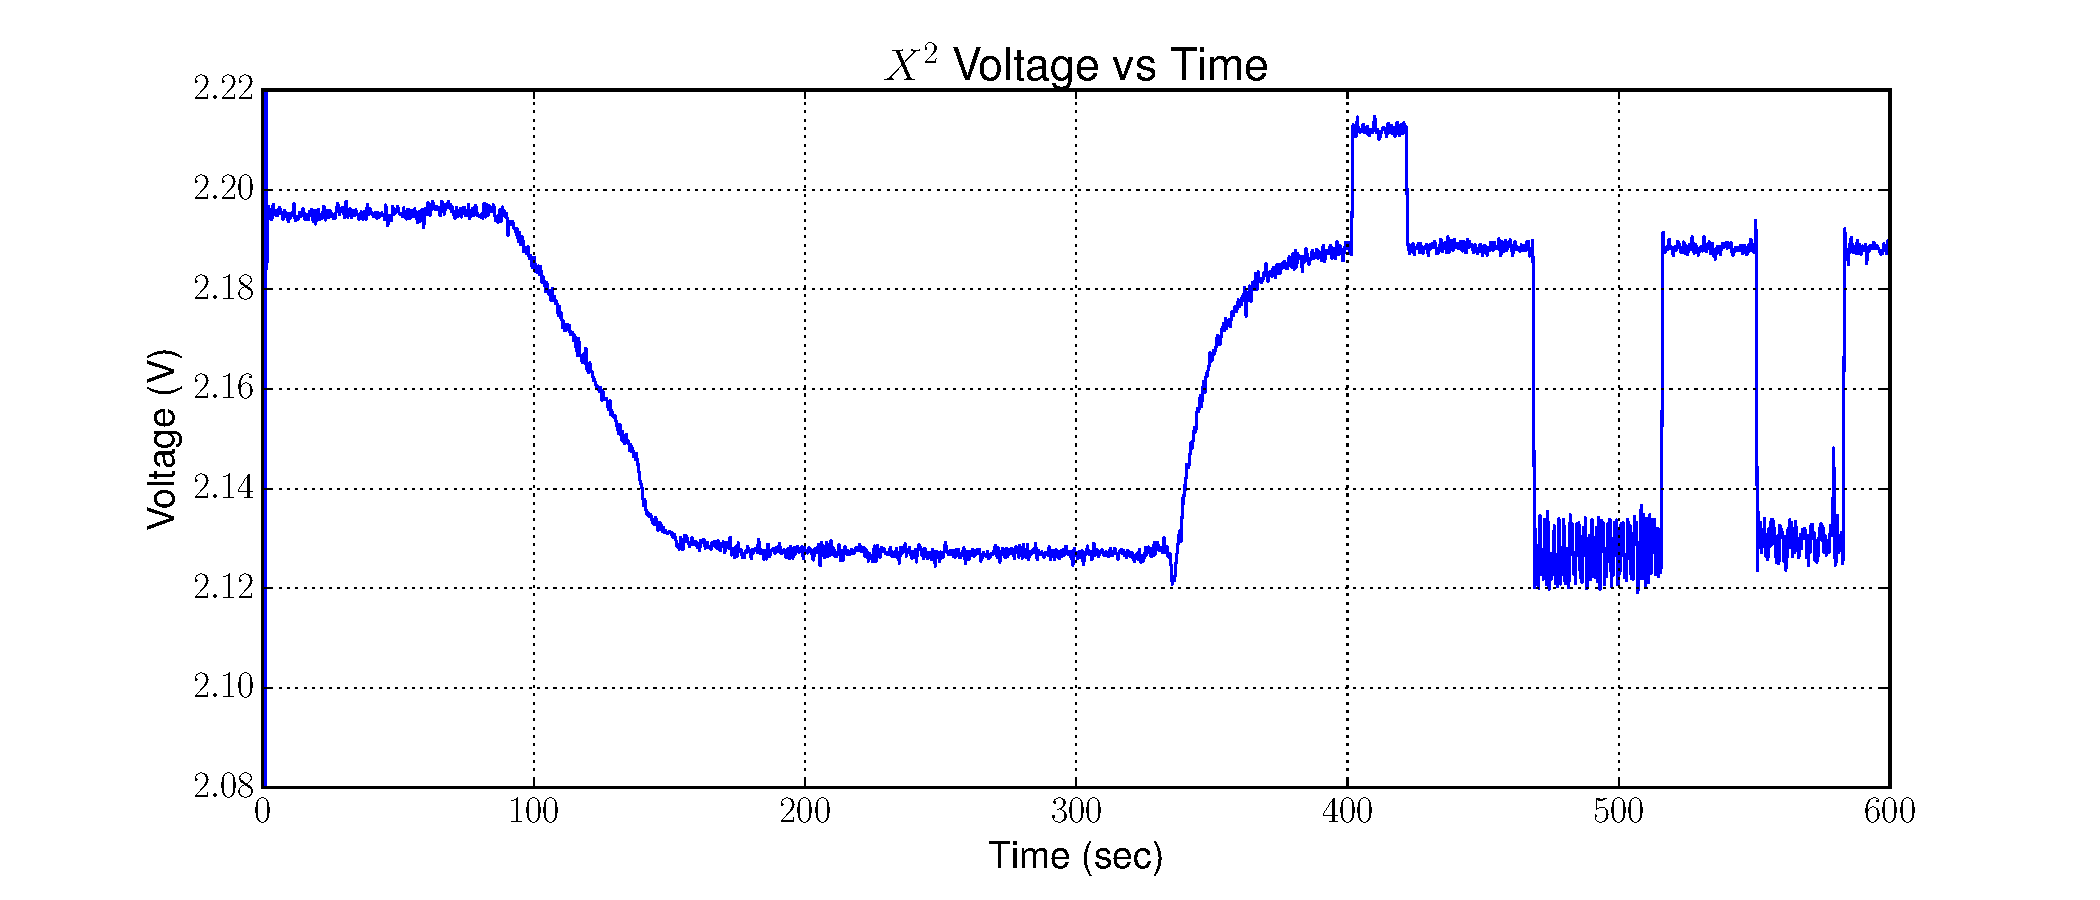
\includegraphics[width=\textwidth]{Experiments/Exp4/x2_voltage.pdf}

\isucaption{Graph showing the raw total power read from the square-law detector with an interfering signal.}
\label{x2_unfilt}
\end{figure}

We can clearly see in both the software defined radio and the square-law detector that there is an interfering signal.  If we now look at the spectrum view on the software defined radio, we can see the signal in questions which is at 1.405 GHz.  Figure \ref{spectrum_interfering} shows us what the software defined radio sees which is a spike at 1.405 GHz.  The square-law detector of course has no frequency information, so our only method to detect an interfering signal is by looking at the total power readings.  In our case there is elevated readings and we can see the spikes in the square-law data.  However, we do not know where in the spectrum the signal is at.

\begin{figure}[h!tb] \centering

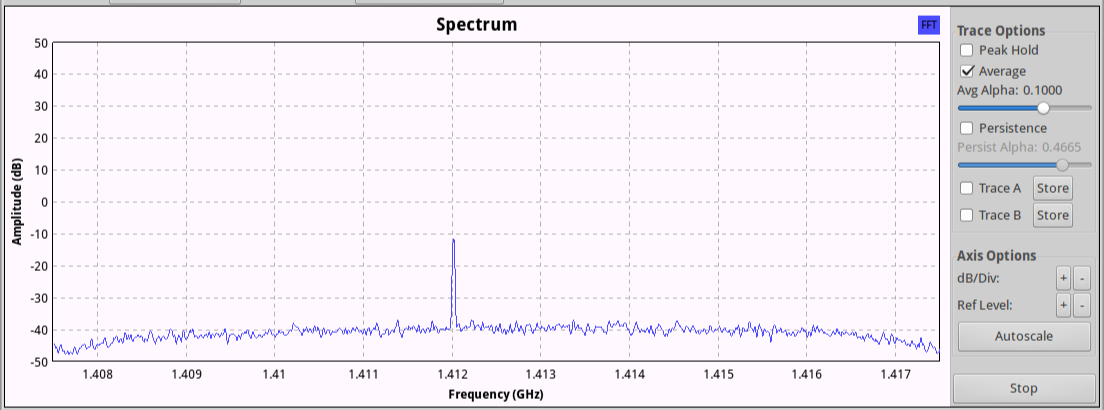
\includegraphics[width=\textwidth]{Images/spectrum_interference.png}

\isucaption{Image showing the spectrum view from the software defined radio}
\label{spectrum_interfering}
\end{figure}

Since we know where the offending signal is, we can now design our filter to filter out this signal.  In our GNURadio program we can specify both the frequency and the bandwidth our band-reject filter that we desire.  Ideally we want to keep the bandwidth of the filter as tight as possible to the offending signal but we also want to make sure our filter is effective in removing the signal.  Figure \ref{spectrum_filter} shows the spectrum display from the software defined radio with the filter now turned on and filtering the offending signal.

\begin{figure}[h!tb] \centering

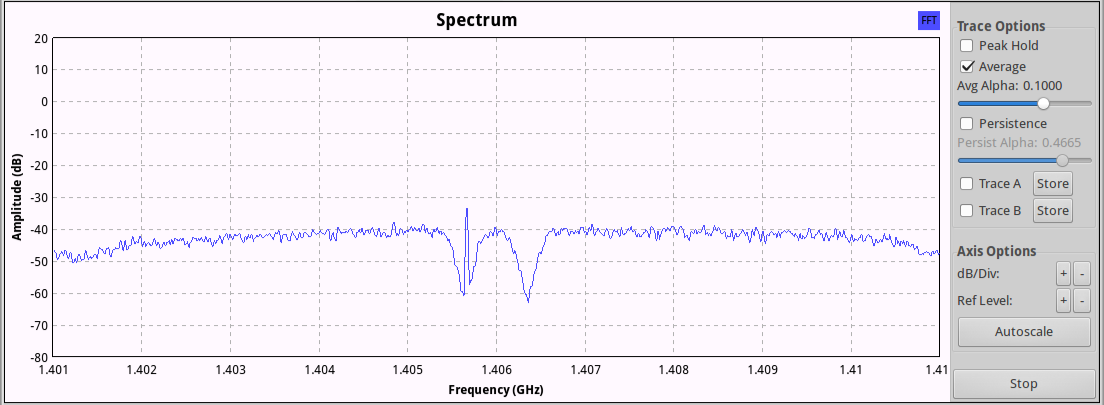
\includegraphics[width=\textwidth]{Images/spectrum_filter.png}

\isucaption{Image showing the software defined radio with the filter on and filtering the offending signal}
\label{spectrum_filter}
\end{figure}

Since we have now removed the offending signal, we will want to re-run our experiment and once again compare the difference between the software defined radio and the square law detector. We can begin by looking at the software defined radio total power readings.  In figure \ref{sdr_calib_filter} we can see a calibrated graph of the noise temperature seen by the software defined radio.  This graph is very similar to the graphs we expect from our total power radiometer.  However, we want to compare this to our square-law detector as well.  

\begin{figure}[h!tb] \centering

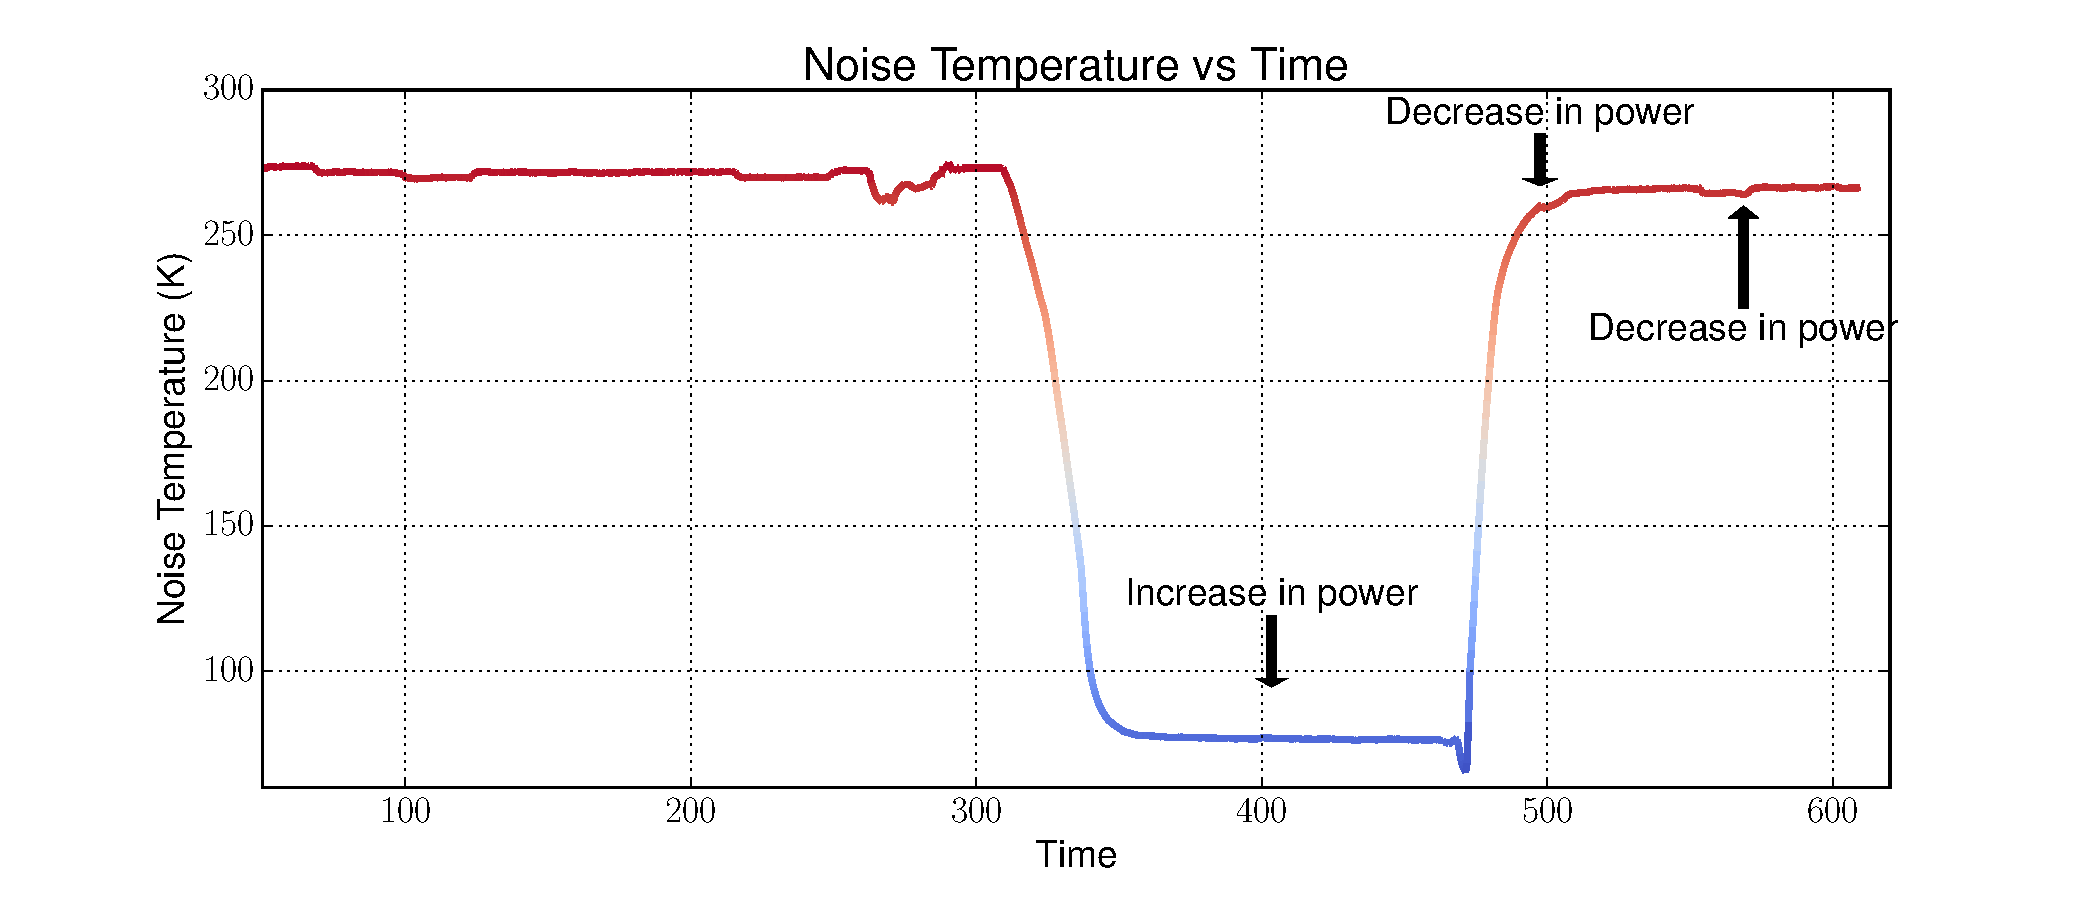
\includegraphics[width=\textwidth]{Experiments/Exp4/calib_filtered.pdf}

\isucaption{Graph showing the calibrated total power readings with the filter removing the offending signal}
\label{sdr_calib_filter}
\end{figure}

Figure \ref{filter_on} now shows both the software defined radio and the square-law detector calibrated total power readings.  In this graph you can see that the software defined radio is able to make normal readings where the square-law detector still shows the changes in amplitude which would make both calibration and obtaining useful data difficult.

\begin{figure}[h!tb] \centering

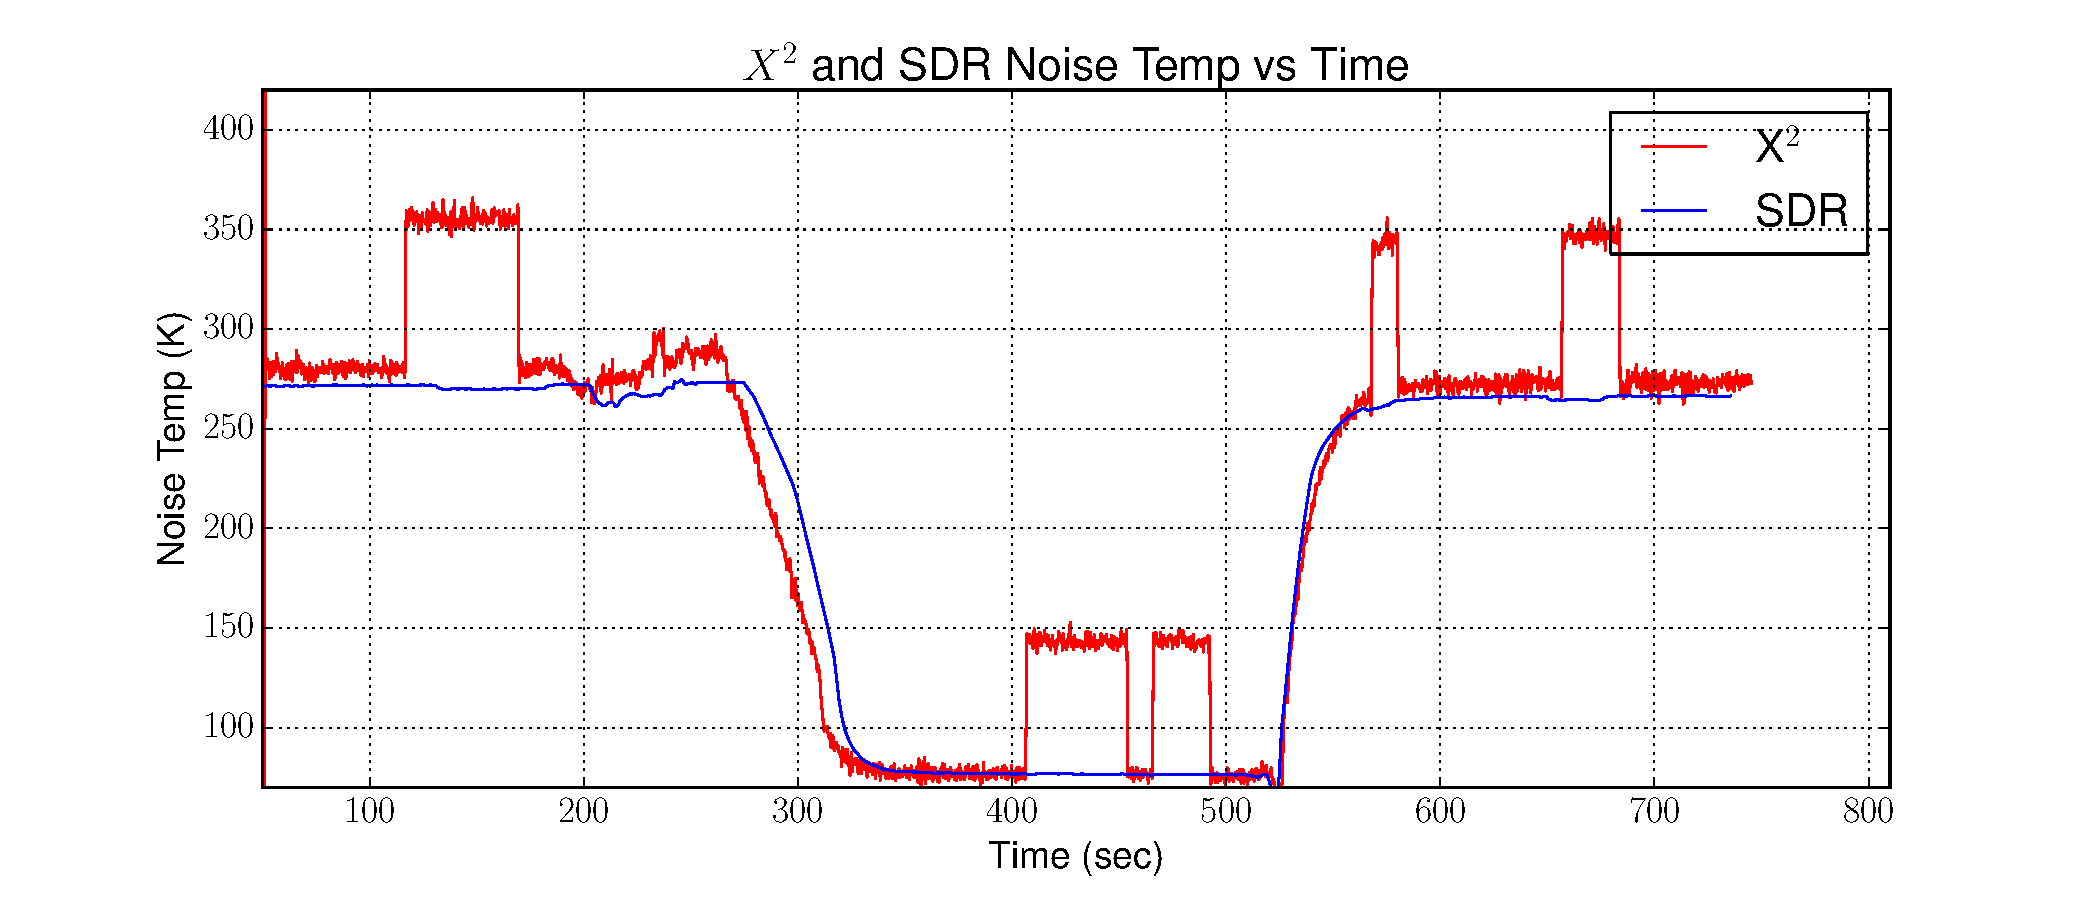
\includegraphics[width=\textwidth]{Experiments/Exp4/calib_filtered_both.pdf}

\isucaption{Image of the offending signal being filtered out by the SDR.  It can be seen that the signal is no longer visible.}
\label{filter_on}
\end{figure}


\section{Further testing}
The software defined radio radiometer can be used in other configurations as well.  Further testing is needed to compare some of these other modes to a traditional radiometer to verify their operation, but in theory these additional configurations should operate the same in a software defined radio as they do with a traditional radiometer.